%
% 2-ritz.tex -- Das Verfahren von Ritz
%
% (c) 2024 Prof Dr Andreas Müller
%
\section{Das Verfahren von Ritz
\label{buch:direkt:section:ritz}}
\kopfrechts{Das Verfahren von Ritz}
Zu einem gegebenen Funktional
\begin{equation}
I(y)
=
\int_{x_1}^{x_2}
L(x,y(x),y'(x))
\,dx
\label{buch:direkt:ritz:eqn:funktional}
\end{equation}
soll eine Funktion $y(x)$ gefunden werden, die das Funktional
extremal macht.

%
% Idee der Methode
%
\subsection{Idee der Methode}
Die Idee des Verfahrens von Ritz
\index{Verfahren!von Ritz}%
\index{Ritz-Verfahren}%
versucht das Extremalproblem für das Funktional $I(y)$ auf ein
endlichdimensionales Problem zu reduzieren, welches dann mit der
vertrauten Gradientmethode von
Abschnitt~\ref{buch:direkt:section:gradient} gelöst werden kann.

%
% Reduktion auf eine endlichdimensionales Problem
%
\subsubsection{Reduktion auf ein endlichdimensionales Problem}
In Abschnitt~\ref{buch:direkt:section:gradient} wurde gezeigt, wie 
Extermalprobleme für endlich viele Variablen zum Beispiel mit der
Gradientabstiegsmethode gelöst werden können.
Diese Methoden sind in dieser Form nicht auf das Variationsproblem
\eqref{buch:direkt:ritz:eqn:funktional} anwendbar, da die Funktion
$y(x)$ nicht nur die Information enthält, die in endlich vielen
Koordinaten $x_1,\dots,x_n$ stecken kann.
Es ist daher nötig, die in Frage kommenden Funktionen durch eine
endlich Zahl von Parametern zu beschreiben.
Man wählt daher Funktionen $\psi_1(x),\dots,\psi_n(x)$ und beschränkt
sich auf Funktion $y(x)$ der Form
\[
y(x)
=
\sum_{k=1}^n
a_k \psi_k(x).
\]
Der Funktionenraum 
\[
B_n
=
\biggl\{
y(x)
=
\sum_{k=1}^n a_k\psi_k(x)
\;
\bigg|
\;
a_1,\dots,a_k\in\mathbb{R}
\biggr\}
\]
ist endlichdimensional und kann durch die Koeffizienten $a_1,\dots,a_n$
parametrisiert werden.
Die Funktionen $\psi_k$ heissen auch die Koordinatenfunktionen und die
$a_k$ die Koordinaten.
Das Funktional $I(y)$ wird jetzt ebenfalls eine Funktion
\[
f(a_1,\dots,a_n)
=
\int_{x_1}^{x_2}
L\biggl(x,
\sum_{k=1}^n a_k\psi_k(x),
\sum_{k=1}^n a_k\psi_k'(x)
\biggr)
\,dx
\]
der Variablen $a_1,\dots,a_n$.
Die Koordinatenfunktionen ermöglichen also, das unendlichdimensionale
Variationsproblem auf ein endlichdimensionales Problem zu reduzieren.

%
% Konvergenz
%
\subsubsection{Konvergenz}
Da der Funktionenraum $B_n$ nur endlichdimensional ist, wird sich darin
im Allgemeinen nur eine Approximation der Lösung des ursprünglichen
Extremalproblems für das Funktional finden lassen.
Je genauer die Koordinatenfunktionen die Lösung zu approximieren gestatten,
desto genauer kann auch der Gradientabstieg die Lösung in $B_n$ zu finden.
Um die Genauigkeit zu steigern, müssen weitere Funktionen zu $B_n$ hinzukommen.
Wir gehen daher im Folgenden von einer Folge von Koordinatenfunktionen
$\psi_k(x)$ mit $k\in \mathbb{N}$ und den Funktionenräumen
\[
B_n
=
\langle \psi_1(x),\dots,\psi_n(x)\rangle
=
\biggl\{
\sum_{k=1}^n a_k^{(n)} \psi_k(x)
\;
\bigg|
\;
a_1^{(n)},\dots,a_n^{(n)}\in\mathbb{R}
\biggr\}
\]
für alle $n\in\mathbb{N}$ aus.
In jedem $B_n$ gibt es eine optimale Lösung
\[
y_n(x)
=
\sum_{k=1}^n a_k^{(n)} \psi_k(x)
\]
Im besten Fall konvergiert nicht nur die Folge $y_n(x)$ gegen die
Funktion $y(x)$ die das Funktional extremal macht, sondern auch
die Folge
\[
a_k^{(k)},
a_k^{(k+1)},
a_k^{(k+2)},
\dots,
a_k^{(k+n)},
\dots
\]
Koeffizienten $a_k^{(k)}$ gegen den Grenzwert $a_k$.
Durch Vergrössern von $n$ kann so eine beliebig genaue Lösung des
ursprünglichen Problems gewonnen werden.
Allerdings ist die Entscheidung, ob die genannten Folgen tatsächlich
konvergieren werden, nicht immer einfach.

%
% Refraktion mit der Methode von Ritz
%
\subsection{Refraktion mit der Methode von Ritz
\label{buch:direkt:ritz:subsection:refraktion}}
In der Übungsaufgabe~\ref{201} wurde das Problem der Refraktion eines
Lichtstrahls in der inhomogenen Atmosphäre untersucht und es wurde als
Euler-Lagrange-Differentialgleichung eine Gleichung gefunden, die nicht
direkt lösbar war.
In diesem Abschnitt versuchen wir das Problem mit dem Verfahren von Ritz
zu lösen.

\begin{aufgabe}
\label{buch:direkt:ritz:aufgabe:lichtstrahl}
Man finde den Weg eines Lichtstrahls durch ein inhomogenes Medium
in der $x$-$y$-Ebene,
dessen Brechungsindex $n(y)=1+\nu y$ ist, der die Zeit zwischen
den Punkten $(0,0)$ und $(\pi,0)$ minimiert.
\end{aufgabe}

Die Lichtgeschwindigkeit ist $c/n(y)$.
Die Zeit $t$, die der Lichtstrahl entlang des Pfades $y(x)$ braucht, ist
daher
\[
t
=
\frac{1}{c}
\int_0^\pi n(y) \sqrt{1+y'(x)^2}.
\]
Dieses Funktional ist also zu minimieren.
Als approximierende Funktionen auf dem Intervall $[0,\pi]$ verwenden 
wir die Funktionen $\psi_k(x) = \sin (2k-1)x$, die Funktion $y(x)$ wird also
in eine Fourier-Sinus-Reihe entwickelt.
Die Approximation $y_n(x)$ mit $n$ Termen ist
\begin{align}
y_n(x)
&=
a_1\sin x
+
a_2\sin 3x
+
\dots
+
a_n\sin (2n-1)x
\notag
\\
&=
\sum_{k=1}^n a_k\sin(2k-1)x
\label{buch:direkt:ritz:bsp:eqn:y}
\intertext{und Ableitung}
y'_n(x)
&=
a_1\cos x
+
3a_2\cos 3x
+
\dots
+
(2n-1)a_n\cos (2n-1)x
\notag
\\
&=
\sum_{k=1}^n (2k-1)a_k\cos(2k-1)x.
\label{buch:direkt:ritz:bsp:eqn:yp}
\end{align}
Die Randbedingung $y_n(0)=y_n(\pi)=0$ ist für alle $n$ automatisch immer
erfüllt, da sie für alle Summanden bereits erfüllt ist.

Für $n=1$ wird das Extremalproblem zu der Aufgabe, den Koeffizienten $a_1$
im Integral
\[
f(a_1)
=
\int_0^\pi (1+\nu a_1\sin x)\sqrt{1+a_1^2\sin^2 x}\,dx
\]
so zu wählen, dass das Minimum erreicht wird.
Leider ist das Integral nicht elementar auswertbar, so dass die Aufgabe
nur numerisch gelöst werden kann.
Dasselbe gilt für die Approximation $n$-ter Ordnung
\[
f_n(a_1,\dots,a_n)
=
\int_0^\pi
(1+\nu y_n(x))
\sqrt{1+y'_n(x)^2}
\,dx.
\]
Davon wird für die Gradientabstiegsmethode der Gradient benötigt,
also die partiellen Ableitungen nach jedem Koeffizienten $a_k$.
Die Ableitung nach $a_k$ kann unter dem Integralzeichen ausgeführt werden
und benötigt die Ableitungen von $y_n(x)$, $y'_n(x)$ und $\sqrt{1+y'_n(x)^2}$
nach $a_k$, die man aus
\eqref{buch:direkt:ritz:bsp:eqn:y}
und
\eqref{buch:direkt:ritz:bsp:eqn:yp}
als
\begin{align*}
\frac{\partial y_n}{\partial a_k}(x)
&=
\sin (2k-1) x
\\
\frac{\partial y'_n}{\partial a_k}(x)
&=
(2k-1)\cos(2k-1)x
\\
\frac{\partial}{\partial a_k}\sqrt{1+y'_n(x)^2}
&=
\frac{y_n'(x)}{\sqrt{1+y_n'(x)^2}}(2k-1)\cos(2k-1)x
\end{align*}
finden kann.
Damit werden die partiellen Ableitungen von $f$ mit der Produktregel
\begin{align}
\frac{\partial f}{\partial a_k}(a_1,\dots,a_n)
&=
\int_0^\pi
\frac{\partial}{\partial a_k}\biggl(
(1+\nu y_n(x))
\sqrt{1+y_n'(x)^2}
\biggr)\,dx
\notag
\\
&=
\int_0^\pi 
\nu
\frac{\partial y_n(x)}{\partial a_k}\sqrt{1+y_n'(x)^2}
+
(1+\nu y_n(x))
\frac{y_n'(x)}{\sqrt{1+y_n'(x)^2}}\frac{\partial y_n'}{\partial a_k}
\,dx
\notag
\\
&=
\int_0^\pi
\nu \sin(2k-1)x \sqrt{1+y_n'(x)^2}
\notag
\\
&\qquad\qquad
+
(1+\nu y_n(x))\frac{y_n'(x)}{\sqrt{1+y_n'(x)^2}}(2k-1)\cos(2k-1)x
\,dx.
\label{buch:direkt:ritz:bsp:eqn:grad}
\end{align}
Der Gradient kann also durch Berechnung der Integrale
\eqref{buch:direkt:ritz:bsp:eqn:grad} ermittelt werden.
Diese Integration ist numerisch leicht möglich.
Damit kann der Gradientabstieg ausgeführt werden.
Die Koeffizienten der Lösung $y_n(x)$ können jeweils als Startwerte
für den weiteren Gradientabstieg zur Lösung $y_{n+1}(x)$ verwendet
werden.
Tabelle~\ref{buch:direkt:ritz:table:koeffizienten} zeigt die gefundenen
Koeffizienten, es ist plausibel, dass sie konvergieren.

Abbildung~\ref{buch:direkt:ritz:fig:ritzloesung} zeigt die visuell
nicht von der mit der Euler-Lagrange-Differential\-glei\-chung
gefundenen Lösung $y_\infty(x)$ unterscheidbaren Lösungen $y_n(x)$ 
des Ritz-Verfahrens.
Die Graphen rechts in der Abbildung zeigen die Fehler der Approximationen
$y_n(x)$.
Man kann ablesen, dass mit nur sechs Termen die Approximation
$y_6(x)$ bereits Fehler $<10^{-3}$ hat.

Für das Refraktionsproblem ist vor allem auch das Ausmass der Lichtbrechung
interessant.
Dieses ist gegeben durch die Steigung der Lösung in den Randpunkten.
Aus Symmetriegründen ist $y'_n(0)=-y'_n(\pi)$.
Tabelle~\ref{buch:direkt:ritz:table:anfangsbed} zeigt die Anfangsbedingung
$y_n(0)$ für die Lösungen des Ritz-Verfahrens wie auch 
$y_\infty(0)$ der Lösung der Euler-Lagrange-Differentialgleichung.
Auch hier ist in Anbetracht der kleinen Anzahl Terme eine erstaunliche
Genauigkeit erreicht worden.

\begin{table}
\def\dglsol{
	({0.0000*\dx},{0.0000*\dy})
	-- ({0.0317*\dx},{-0.0106*\dy})
	-- ({0.0635*\dx},{-0.0210*\dy})
	-- ({0.0952*\dx},{-0.0311*\dy})
	-- ({0.1269*\dx},{-0.0411*\dy})
	-- ({0.1587*\dx},{-0.0508*\dy})
	-- ({0.1904*\dx},{-0.0603*\dy})
	-- ({0.2221*\dx},{-0.0695*\dy})
	-- ({0.2539*\dx},{-0.0786*\dy})
	-- ({0.2856*\dx},{-0.0874*\dy})
	-- ({0.3173*\dx},{-0.0960*\dy})
	-- ({0.3491*\dx},{-0.1044*\dy})
	-- ({0.3808*\dx},{-0.1126*\dy})
	-- ({0.4125*\dx},{-0.1205*\dy})
	-- ({0.4443*\dx},{-0.1282*\dy})
	-- ({0.4760*\dx},{-0.1358*\dy})
	-- ({0.5077*\dx},{-0.1430*\dy})
	-- ({0.5395*\dx},{-0.1501*\dy})
	-- ({0.5712*\dx},{-0.1570*\dy})
	-- ({0.6029*\dx},{-0.1636*\dy})
	-- ({0.6347*\dx},{-0.1700*\dy})
	-- ({0.6664*\dx},{-0.1762*\dy})
	-- ({0.6981*\dx},{-0.1822*\dy})
	-- ({0.7299*\dx},{-0.1880*\dy})
	-- ({0.7616*\dx},{-0.1935*\dy})
	-- ({0.7933*\dx},{-0.1989*\dy})
	-- ({0.8251*\dx},{-0.2040*\dy})
	-- ({0.8568*\dx},{-0.2089*\dy})
	-- ({0.8885*\dx},{-0.2136*\dy})
	-- ({0.9203*\dx},{-0.2181*\dy})
	-- ({0.9520*\dx},{-0.2224*\dy})
	-- ({0.9837*\dx},{-0.2264*\dy})
	-- ({1.0155*\dx},{-0.2302*\dy})
	-- ({1.0472*\dx},{-0.2339*\dy})
	-- ({1.0789*\dx},{-0.2373*\dy})
	-- ({1.1107*\dx},{-0.2405*\dy})
	-- ({1.1424*\dx},{-0.2434*\dy})
	-- ({1.1741*\dx},{-0.2462*\dy})
	-- ({1.2059*\dx},{-0.2488*\dy})
	-- ({1.2376*\dx},{-0.2511*\dy})
	-- ({1.2693*\dx},{-0.2532*\dy})
	-- ({1.3011*\dx},{-0.2551*\dy})
	-- ({1.3328*\dx},{-0.2568*\dy})
	-- ({1.3645*\dx},{-0.2583*\dy})
	-- ({1.3963*\dx},{-0.2596*\dy})
	-- ({1.4280*\dx},{-0.2607*\dy})
	-- ({1.4597*\dx},{-0.2615*\dy})
	-- ({1.4915*\dx},{-0.2622*\dy})
	-- ({1.5232*\dx},{-0.2626*\dy})
	-- ({1.5549*\dx},{-0.2628*\dy})
	-- ({1.5867*\dx},{-0.2628*\dy})
	-- ({1.6184*\dx},{-0.2626*\dy})
	-- ({1.6501*\dx},{-0.2622*\dy})
	-- ({1.6819*\dx},{-0.2615*\dy})
	-- ({1.7136*\dx},{-0.2607*\dy})
	-- ({1.7453*\dx},{-0.2596*\dy})
	-- ({1.7771*\dx},{-0.2583*\dy})
	-- ({1.8088*\dx},{-0.2568*\dy})
	-- ({1.8405*\dx},{-0.2551*\dy})
	-- ({1.8723*\dx},{-0.2532*\dy})
	-- ({1.9040*\dx},{-0.2511*\dy})
	-- ({1.9357*\dx},{-0.2488*\dy})
	-- ({1.9675*\dx},{-0.2462*\dy})
	-- ({1.9992*\dx},{-0.2434*\dy})
	-- ({2.0309*\dx},{-0.2405*\dy})
	-- ({2.0627*\dx},{-0.2373*\dy})
	-- ({2.0944*\dx},{-0.2339*\dy})
	-- ({2.1261*\dx},{-0.2302*\dy})
	-- ({2.1579*\dx},{-0.2264*\dy})
	-- ({2.1896*\dx},{-0.2224*\dy})
	-- ({2.2213*\dx},{-0.2181*\dy})
	-- ({2.2531*\dx},{-0.2136*\dy})
	-- ({2.2848*\dx},{-0.2089*\dy})
	-- ({2.3165*\dx},{-0.2040*\dy})
	-- ({2.3483*\dx},{-0.1989*\dy})
	-- ({2.3800*\dx},{-0.1935*\dy})
	-- ({2.4117*\dx},{-0.1880*\dy})
	-- ({2.4435*\dx},{-0.1822*\dy})
	-- ({2.4752*\dx},{-0.1762*\dy})
	-- ({2.5069*\dx},{-0.1700*\dy})
	-- ({2.5387*\dx},{-0.1636*\dy})
	-- ({2.5704*\dx},{-0.1570*\dy})
	-- ({2.6021*\dx},{-0.1501*\dy})
	-- ({2.6339*\dx},{-0.1430*\dy})
	-- ({2.6656*\dx},{-0.1358*\dy})
	-- ({2.6973*\dx},{-0.1282*\dy})
	-- ({2.7291*\dx},{-0.1205*\dy})
	-- ({2.7608*\dx},{-0.1126*\dy})
	-- ({2.7925*\dx},{-0.1044*\dy})
	-- ({2.8243*\dx},{-0.0960*\dy})
	-- ({2.8560*\dx},{-0.0874*\dy})
	-- ({2.8877*\dx},{-0.0786*\dy})
	-- ({2.9195*\dx},{-0.0695*\dy})
	-- ({2.9512*\dx},{-0.0603*\dy})
	-- ({2.9829*\dx},{-0.0508*\dy})
	-- ({3.0147*\dx},{-0.0411*\dy})
	-- ({3.0464*\dx},{-0.0311*\dy})
	-- ({3.0781*\dx},{-0.0210*\dy})
	-- ({3.1099*\dx},{-0.0106*\dy})
	-- ({3.1416*\dx},{-0.0000*\dy})
}
\def\lone{
	({0.00000*\dx},{0.00000*\dy})
	-- ({0.03173*\dx},{-0.00860*\dy})
	-- ({0.06347*\dx},{-0.01719*\dy})
	-- ({0.09520*\dx},{-0.02576*\dy})
	-- ({0.12693*\dx},{-0.03430*\dy})
	-- ({0.15867*\dx},{-0.04281*\dy})
	-- ({0.19040*\dx},{-0.05128*\dy})
	-- ({0.22213*\dx},{-0.05970*\dy})
	-- ({0.25387*\dx},{-0.06805*\dy})
	-- ({0.28560*\dx},{-0.07634*\dy})
	-- ({0.31733*\dx},{-0.08455*\dy})
	-- ({0.34907*\dx},{-0.09268*\dy})
	-- ({0.38080*\dx},{-0.10071*\dy})
	-- ({0.41253*\dx},{-0.10864*\dy})
	-- ({0.44427*\dx},{-0.11646*\dy})
	-- ({0.47600*\dx},{-0.12416*\dy})
	-- ({0.50773*\dx},{-0.13174*\dy})
	-- ({0.53947*\dx},{-0.13919*\dy})
	-- ({0.57120*\dx},{-0.14650*\dy})
	-- ({0.60293*\dx},{-0.15365*\dy})
	-- ({0.63467*\dx},{-0.16066*\dy})
	-- ({0.66640*\dx},{-0.16750*\dy})
	-- ({0.69813*\dx},{-0.17417*\dy})
	-- ({0.72986*\dx},{-0.18067*\dy})
	-- ({0.76160*\dx},{-0.18699*\dy})
	-- ({0.79333*\dx},{-0.19312*\dy})
	-- ({0.82506*\dx},{-0.19905*\dy})
	-- ({0.85680*\dx},{-0.20478*\dy})
	-- ({0.88853*\dx},{-0.21031*\dy})
	-- ({0.92026*\dx},{-0.21562*\dy})
	-- ({0.95200*\dx},{-0.22072*\dy})
	-- ({0.98373*\dx},{-0.22560*\dy})
	-- ({1.01546*\dx},{-0.23025*\dy})
	-- ({1.04720*\dx},{-0.23466*\dy})
	-- ({1.07893*\dx},{-0.23884*\dy})
	-- ({1.11066*\dx},{-0.24278*\dy})
	-- ({1.14240*\dx},{-0.24648*\dy})
	-- ({1.17413*\dx},{-0.24993*\dy})
	-- ({1.20586*\dx},{-0.25312*\dy})
	-- ({1.23760*\dx},{-0.25606*\dy})
	-- ({1.26933*\dx},{-0.25875*\dy})
	-- ({1.30106*\dx},{-0.26117*\dy})
	-- ({1.33280*\dx},{-0.26333*\dy})
	-- ({1.36453*\dx},{-0.26522*\dy})
	-- ({1.39626*\dx},{-0.26685*\dy})
	-- ({1.42800*\dx},{-0.26821*\dy})
	-- ({1.45973*\dx},{-0.26930*\dy})
	-- ({1.49146*\dx},{-0.27011*\dy})
	-- ({1.52320*\dx},{-0.27066*\dy})
	-- ({1.55493*\dx},{-0.27093*\dy})
	-- ({1.58666*\dx},{-0.27093*\dy})
	-- ({1.61840*\dx},{-0.27066*\dy})
	-- ({1.65013*\dx},{-0.27011*\dy})
	-- ({1.68186*\dx},{-0.26930*\dy})
	-- ({1.71360*\dx},{-0.26821*\dy})
	-- ({1.74533*\dx},{-0.26685*\dy})
	-- ({1.77706*\dx},{-0.26522*\dy})
	-- ({1.80880*\dx},{-0.26333*\dy})
	-- ({1.84053*\dx},{-0.26117*\dy})
	-- ({1.87226*\dx},{-0.25875*\dy})
	-- ({1.90400*\dx},{-0.25606*\dy})
	-- ({1.93573*\dx},{-0.25312*\dy})
	-- ({1.96746*\dx},{-0.24993*\dy})
	-- ({1.99920*\dx},{-0.24648*\dy})
	-- ({2.03093*\dx},{-0.24278*\dy})
	-- ({2.06266*\dx},{-0.23884*\dy})
	-- ({2.09440*\dx},{-0.23466*\dy})
	-- ({2.12613*\dx},{-0.23025*\dy})
	-- ({2.15786*\dx},{-0.22560*\dy})
	-- ({2.18959*\dx},{-0.22072*\dy})
	-- ({2.22133*\dx},{-0.21562*\dy})
	-- ({2.25306*\dx},{-0.21031*\dy})
	-- ({2.28479*\dx},{-0.20478*\dy})
	-- ({2.31653*\dx},{-0.19905*\dy})
	-- ({2.34826*\dx},{-0.19312*\dy})
	-- ({2.37999*\dx},{-0.18699*\dy})
	-- ({2.41173*\dx},{-0.18067*\dy})
	-- ({2.44346*\dx},{-0.17417*\dy})
	-- ({2.47519*\dx},{-0.16750*\dy})
	-- ({2.50693*\dx},{-0.16066*\dy})
	-- ({2.53866*\dx},{-0.15365*\dy})
	-- ({2.57039*\dx},{-0.14650*\dy})
	-- ({2.60213*\dx},{-0.13919*\dy})
	-- ({2.63386*\dx},{-0.13174*\dy})
	-- ({2.66559*\dx},{-0.12416*\dy})
	-- ({2.69733*\dx},{-0.11646*\dy})
	-- ({2.72906*\dx},{-0.10864*\dy})
	-- ({2.76079*\dx},{-0.10071*\dy})
	-- ({2.79253*\dx},{-0.09268*\dy})
	-- ({2.82426*\dx},{-0.08455*\dy})
	-- ({2.85599*\dx},{-0.07634*\dy})
	-- ({2.88773*\dx},{-0.06805*\dy})
	-- ({2.91946*\dx},{-0.05970*\dy})
	-- ({2.95119*\dx},{-0.05128*\dy})
	-- ({2.98293*\dx},{-0.04281*\dy})
	-- ({3.01466*\dx},{-0.03430*\dy})
	-- ({3.04639*\dx},{-0.02576*\dy})
	-- ({3.07813*\dx},{-0.01719*\dy})
	-- ({3.10986*\dx},{-0.00860*\dy})
	-- ({3.14159*\dx},{-0.00000*\dy})
}
\def\eone{
	({0.00000*\dx},{0.0000*\dy})
	-- ({0.03173*\dx},{0.20070*\dy})
	-- ({0.06347*\dx},{0.37988*\dy})
	-- ({0.09520*\dx},{0.53844*\dy})
	-- ({0.12693*\dx},{0.67731*\dy})
	-- ({0.15867*\dx},{0.79737*\dy})
	-- ({0.19040*\dx},{0.89953*\dy})
	-- ({0.22213*\dx},{0.98469*\dy})
	-- ({0.25387*\dx},{1.05374*\dy})
	-- ({0.28560*\dx},{1.10756*\dy})
	-- ({0.31733*\dx},{1.14702*\dy})
	-- ({0.34907*\dx},{1.17298*\dy})
	-- ({0.38080*\dx},{1.18631*\dy})
	-- ({0.41253*\dx},{1.18785*\dy})
	-- ({0.44427*\dx},{1.17843*\dy})
	-- ({0.47600*\dx},{1.15888*\dy})
	-- ({0.50773*\dx},{1.13000*\dy})
	-- ({0.53947*\dx},{1.09259*\dy})
	-- ({0.57120*\dx},{1.04743*\dy})
	-- ({0.60293*\dx},{0.99529*\dy})
	-- ({0.63467*\dx},{0.93692*\dy})
	-- ({0.66640*\dx},{0.87306*\dy})
	-- ({0.69813*\dx},{0.80441*\dy})
	-- ({0.72986*\dx},{0.73168*\dy})
	-- ({0.76160*\dx},{0.65555*\dy})
	-- ({0.79333*\dx},{0.57668*\dy})
	-- ({0.82506*\dx},{0.49571*\dy})
	-- ({0.85680*\dx},{0.41326*\dy})
	-- ({0.88853*\dx},{0.32994*\dy})
	-- ({0.92026*\dx},{0.24631*\dy})
	-- ({0.95200*\dx},{0.16293*\dy})
	-- ({0.98373*\dx},{0.08034*\dy})
	-- ({1.01546*\dx},{-0.00096*\dy})
	-- ({1.04720*\dx},{-0.08047*\dy})
	-- ({1.07893*\dx},{-0.15775*\dy})
	-- ({1.11066*\dx},{-0.23234*\dy})
	-- ({1.14240*\dx},{-0.30385*\dy})
	-- ({1.17413*\dx},{-0.37189*\dy})
	-- ({1.20586*\dx},{-0.43609*\dy})
	-- ({1.23760*\dx},{-0.49612*\dy})
	-- ({1.26933*\dx},{-0.55168*\dy})
	-- ({1.30106*\dx},{-0.60249*\dy})
	-- ({1.33280*\dx},{-0.64829*\dy})
	-- ({1.36453*\dx},{-0.68887*\dy})
	-- ({1.39626*\dx},{-0.72401*\dy})
	-- ({1.42800*\dx},{-0.75356*\dy})
	-- ({1.45973*\dx},{-0.77736*\dy})
	-- ({1.49146*\dx},{-0.79532*\dy})
	-- ({1.52320*\dx},{-0.80734*\dy})
	-- ({1.55493*\dx},{-0.81336*\dy})
	-- ({1.58666*\dx},{-0.81336*\dy})
	-- ({1.61840*\dx},{-0.80734*\dy})
	-- ({1.65013*\dx},{-0.79532*\dy})
	-- ({1.68186*\dx},{-0.77736*\dy})
	-- ({1.71360*\dx},{-0.75355*\dy})
	-- ({1.74533*\dx},{-0.72401*\dy})
	-- ({1.77706*\dx},{-0.68886*\dy})
	-- ({1.80880*\dx},{-0.64829*\dy})
	-- ({1.84053*\dx},{-0.60249*\dy})
	-- ({1.87226*\dx},{-0.55168*\dy})
	-- ({1.90400*\dx},{-0.49612*\dy})
	-- ({1.93573*\dx},{-0.43608*\dy})
	-- ({1.96746*\dx},{-0.37188*\dy})
	-- ({1.99920*\dx},{-0.30384*\dy})
	-- ({2.03093*\dx},{-0.23233*\dy})
	-- ({2.06266*\dx},{-0.15774*\dy})
	-- ({2.09440*\dx},{-0.08046*\dy})
	-- ({2.12613*\dx},{-0.00095*\dy})
	-- ({2.15786*\dx},{0.08035*\dy})
	-- ({2.18959*\dx},{0.16294*\dy})
	-- ({2.22133*\dx},{0.24632*\dy})
	-- ({2.25306*\dx},{0.32995*\dy})
	-- ({2.28479*\dx},{0.41328*\dy})
	-- ({2.31653*\dx},{0.49573*\dy})
	-- ({2.34826*\dx},{0.57670*\dy})
	-- ({2.37999*\dx},{0.65557*\dy})
	-- ({2.41173*\dx},{0.73170*\dy})
	-- ({2.44346*\dx},{0.80443*\dy})
	-- ({2.47519*\dx},{0.87307*\dy})
	-- ({2.50693*\dx},{0.93694*\dy})
	-- ({2.53866*\dx},{0.99531*\dy})
	-- ({2.57039*\dx},{1.04745*\dy})
	-- ({2.60213*\dx},{1.09261*\dy})
	-- ({2.63386*\dx},{1.13002*\dy})
	-- ({2.66559*\dx},{1.15890*\dy})
	-- ({2.69733*\dx},{1.17845*\dy})
	-- ({2.72906*\dx},{1.18787*\dy})
	-- ({2.76079*\dx},{1.18634*\dy})
	-- ({2.79253*\dx},{1.17301*\dy})
	-- ({2.82426*\dx},{1.14704*\dy})
	-- ({2.85599*\dx},{1.10758*\dy})
	-- ({2.88773*\dx},{1.05377*\dy})
	-- ({2.91946*\dx},{0.98472*\dy})
	-- ({2.95119*\dx},{0.89956*\dy})
	-- ({2.98293*\dx},{0.79739*\dy})
	-- ({3.01466*\dx},{0.67733*\dy})
	-- ({3.04639*\dx},{0.53847*\dy})
	-- ({3.07813*\dx},{0.37991*\dy})
	-- ({3.10986*\dx},{0.20073*\dy})
	-- ({3.14159*\dx},{0.00003*\dy})
}
\def\ltwo{
	({0.00000*\dx},{0.00000*\dy})
	-- ({0.03173*\dx},{-0.00960*\dy})
	-- ({0.06347*\dx},{-0.01918*\dy})
	-- ({0.09520*\dx},{-0.02873*\dy})
	-- ({0.12693*\dx},{-0.03822*\dy})
	-- ({0.15867*\dx},{-0.04765*\dy})
	-- ({0.19040*\dx},{-0.05699*\dy})
	-- ({0.22213*\dx},{-0.06622*\dy})
	-- ({0.25387*\dx},{-0.07534*\dy})
	-- ({0.28560*\dx},{-0.08433*\dy})
	-- ({0.31733*\dx},{-0.09316*\dy})
	-- ({0.34907*\dx},{-0.10184*\dy})
	-- ({0.38080*\dx},{-0.11034*\dy})
	-- ({0.41253*\dx},{-0.11865*\dy})
	-- ({0.44427*\dx},{-0.12677*\dy})
	-- ({0.47600*\dx},{-0.13468*\dy})
	-- ({0.50773*\dx},{-0.14236*\dy})
	-- ({0.53947*\dx},{-0.14982*\dy})
	-- ({0.57120*\dx},{-0.15705*\dy})
	-- ({0.60293*\dx},{-0.16404*\dy})
	-- ({0.63467*\dx},{-0.17078*\dy})
	-- ({0.66640*\dx},{-0.17727*\dy})
	-- ({0.69813*\dx},{-0.18350*\dy})
	-- ({0.72986*\dx},{-0.18948*\dy})
	-- ({0.76160*\dx},{-0.19520*\dy})
	-- ({0.79333*\dx},{-0.20066*\dy})
	-- ({0.82506*\dx},{-0.20586*\dy})
	-- ({0.85680*\dx},{-0.21080*\dy})
	-- ({0.88853*\dx},{-0.21549*\dy})
	-- ({0.92026*\dx},{-0.21992*\dy})
	-- ({0.95200*\dx},{-0.22409*\dy})
	-- ({0.98373*\dx},{-0.22802*\dy})
	-- ({1.01546*\dx},{-0.23170*\dy})
	-- ({1.04720*\dx},{-0.23514*\dy})
	-- ({1.07893*\dx},{-0.23835*\dy})
	-- ({1.11066*\dx},{-0.24132*\dy})
	-- ({1.14240*\dx},{-0.24406*\dy})
	-- ({1.17413*\dx},{-0.24659*\dy})
	-- ({1.20586*\dx},{-0.24889*\dy})
	-- ({1.23760*\dx},{-0.25098*\dy})
	-- ({1.26933*\dx},{-0.25287*\dy})
	-- ({1.30106*\dx},{-0.25455*\dy})
	-- ({1.33280*\dx},{-0.25603*\dy})
	-- ({1.36453*\dx},{-0.25732*\dy})
	-- ({1.39626*\dx},{-0.25842*\dy})
	-- ({1.42800*\dx},{-0.25933*\dy})
	-- ({1.45973*\dx},{-0.26005*\dy})
	-- ({1.49146*\dx},{-0.26060*\dy})
	-- ({1.52320*\dx},{-0.26096*\dy})
	-- ({1.55493*\dx},{-0.26114*\dy})
	-- ({1.58666*\dx},{-0.26114*\dy})
	-- ({1.61840*\dx},{-0.26096*\dy})
	-- ({1.65013*\dx},{-0.26060*\dy})
	-- ({1.68186*\dx},{-0.26005*\dy})
	-- ({1.71360*\dx},{-0.25933*\dy})
	-- ({1.74533*\dx},{-0.25842*\dy})
	-- ({1.77706*\dx},{-0.25732*\dy})
	-- ({1.80880*\dx},{-0.25603*\dy})
	-- ({1.84053*\dx},{-0.25455*\dy})
	-- ({1.87226*\dx},{-0.25287*\dy})
	-- ({1.90400*\dx},{-0.25098*\dy})
	-- ({1.93573*\dx},{-0.24889*\dy})
	-- ({1.96746*\dx},{-0.24659*\dy})
	-- ({1.99920*\dx},{-0.24406*\dy})
	-- ({2.03093*\dx},{-0.24132*\dy})
	-- ({2.06266*\dx},{-0.23835*\dy})
	-- ({2.09440*\dx},{-0.23514*\dy})
	-- ({2.12613*\dx},{-0.23170*\dy})
	-- ({2.15786*\dx},{-0.22802*\dy})
	-- ({2.18959*\dx},{-0.22409*\dy})
	-- ({2.22133*\dx},{-0.21992*\dy})
	-- ({2.25306*\dx},{-0.21549*\dy})
	-- ({2.28479*\dx},{-0.21080*\dy})
	-- ({2.31653*\dx},{-0.20586*\dy})
	-- ({2.34826*\dx},{-0.20066*\dy})
	-- ({2.37999*\dx},{-0.19520*\dy})
	-- ({2.41173*\dx},{-0.18948*\dy})
	-- ({2.44346*\dx},{-0.18350*\dy})
	-- ({2.47519*\dx},{-0.17727*\dy})
	-- ({2.50693*\dx},{-0.17078*\dy})
	-- ({2.53866*\dx},{-0.16404*\dy})
	-- ({2.57039*\dx},{-0.15705*\dy})
	-- ({2.60213*\dx},{-0.14982*\dy})
	-- ({2.63386*\dx},{-0.14236*\dy})
	-- ({2.66559*\dx},{-0.13468*\dy})
	-- ({2.69733*\dx},{-0.12677*\dy})
	-- ({2.72906*\dx},{-0.11865*\dy})
	-- ({2.76079*\dx},{-0.11034*\dy})
	-- ({2.79253*\dx},{-0.10184*\dy})
	-- ({2.82426*\dx},{-0.09316*\dy})
	-- ({2.85599*\dx},{-0.08433*\dy})
	-- ({2.88773*\dx},{-0.07534*\dy})
	-- ({2.91946*\dx},{-0.06622*\dy})
	-- ({2.95119*\dx},{-0.05699*\dy})
	-- ({2.98293*\dx},{-0.04765*\dy})
	-- ({3.01466*\dx},{-0.03822*\dy})
	-- ({3.04639*\dx},{-0.02873*\dy})
	-- ({3.07813*\dx},{-0.01918*\dy})
	-- ({3.10986*\dx},{-0.00960*\dy})
	-- ({3.14159*\dx},{-0.00000*\dy})
}
\def\etwo{
	({0.00000*\dx},{0.0000*\dy})
	-- ({0.03173*\dx},{0.10044*\dy})
	-- ({0.06347*\dx},{0.18025*\dy})
	-- ({0.09520*\dx},{0.24122*\dy})
	-- ({0.12693*\dx},{0.28514*\dy})
	-- ({0.15867*\dx},{0.31376*\dy})
	-- ({0.19040*\dx},{0.32879*\dy})
	-- ({0.22213*\dx},{0.33190*\dy})
	-- ({0.25387*\dx},{0.32471*\dy})
	-- ({0.28560*\dx},{0.30877*\dy})
	-- ({0.31733*\dx},{0.28559*\dy})
	-- ({0.34907*\dx},{0.25658*\dy})
	-- ({0.38080*\dx},{0.22308*\dy})
	-- ({0.41253*\dx},{0.18634*\dy})
	-- ({0.44427*\dx},{0.14754*\dy})
	-- ({0.47600*\dx},{0.10775*\dy})
	-- ({0.50773*\dx},{0.06794*\dy})
	-- ({0.53947*\dx},{0.02901*\dy})
	-- ({0.57120*\dx},{-0.00827*\dy})
	-- ({0.60293*\dx},{-0.04321*\dy})
	-- ({0.63467*\dx},{-0.07523*\dy})
	-- ({0.66640*\dx},{-0.10384*\dy})
	-- ({0.69813*\dx},{-0.12867*\dy})
	-- ({0.72986*\dx},{-0.14941*\dy})
	-- ({0.76160*\dx},{-0.16587*\dy})
	-- ({0.79333*\dx},{-0.17794*\dy})
	-- ({0.82506*\dx},{-0.18560*\dy})
	-- ({0.85680*\dx},{-0.18889*\dy})
	-- ({0.88853*\dx},{-0.18794*\dy})
	-- ({0.92026*\dx},{-0.18296*\dy})
	-- ({0.95200*\dx},{-0.17419*\dy})
	-- ({0.98373*\dx},{-0.16194*\dy})
	-- ({1.01546*\dx},{-0.14657*\dy})
	-- ({1.04720*\dx},{-0.12849*\dy})
	-- ({1.07893*\dx},{-0.10811*\dy})
	-- ({1.11066*\dx},{-0.08590*\dy})
	-- ({1.14240*\dx},{-0.06233*\dy})
	-- ({1.17413*\dx},{-0.03788*\dy})
	-- ({1.20586*\dx},{-0.01303*\dy})
	-- ({1.23760*\dx},{0.01173*\dy})
	-- ({1.26933*\dx},{0.03595*\dy})
	-- ({1.30106*\dx},{0.05918*\dy})
	-- ({1.33280*\dx},{0.08099*\dy})
	-- ({1.36453*\dx},{0.10099*\dy})
	-- ({1.39626*\dx},{0.11883*\dy})
	-- ({1.42800*\dx},{0.13419*\dy})
	-- ({1.45973*\dx},{0.14681*\dy})
	-- ({1.49146*\dx},{0.15647*\dy})
	-- ({1.52320*\dx},{0.16301*\dy})
	-- ({1.55493*\dx},{0.16630*\dy})
	-- ({1.58666*\dx},{0.16630*\dy})
	-- ({1.61840*\dx},{0.16301*\dy})
	-- ({1.65013*\dx},{0.15647*\dy})
	-- ({1.68186*\dx},{0.14681*\dy})
	-- ({1.71360*\dx},{0.13419*\dy})
	-- ({1.74533*\dx},{0.11883*\dy})
	-- ({1.77706*\dx},{0.10099*\dy})
	-- ({1.80880*\dx},{0.08099*\dy})
	-- ({1.84053*\dx},{0.05918*\dy})
	-- ({1.87226*\dx},{0.03596*\dy})
	-- ({1.90400*\dx},{0.01174*\dy})
	-- ({1.93573*\dx},{-0.01303*\dy})
	-- ({1.96746*\dx},{-0.03787*\dy})
	-- ({1.99920*\dx},{-0.06233*\dy})
	-- ({2.03093*\dx},{-0.08590*\dy})
	-- ({2.06266*\dx},{-0.10810*\dy})
	-- ({2.09440*\dx},{-0.12848*\dy})
	-- ({2.12613*\dx},{-0.14656*\dy})
	-- ({2.15786*\dx},{-0.16193*\dy})
	-- ({2.18959*\dx},{-0.17417*\dy})
	-- ({2.22133*\dx},{-0.18294*\dy})
	-- ({2.25306*\dx},{-0.18793*\dy})
	-- ({2.28479*\dx},{-0.18888*\dy})
	-- ({2.31653*\dx},{-0.18558*\dy})
	-- ({2.34826*\dx},{-0.17793*\dy})
	-- ({2.37999*\dx},{-0.16586*\dy})
	-- ({2.41173*\dx},{-0.14939*\dy})
	-- ({2.44346*\dx},{-0.12865*\dy})
	-- ({2.47519*\dx},{-0.10383*\dy})
	-- ({2.50693*\dx},{-0.07521*\dy})
	-- ({2.53866*\dx},{-0.04319*\dy})
	-- ({2.57039*\dx},{-0.00825*\dy})
	-- ({2.60213*\dx},{0.02903*\dy})
	-- ({2.63386*\dx},{0.06796*\dy})
	-- ({2.66559*\dx},{0.10777*\dy})
	-- ({2.69733*\dx},{0.14756*\dy})
	-- ({2.72906*\dx},{0.18637*\dy})
	-- ({2.76079*\dx},{0.22310*\dy})
	-- ({2.79253*\dx},{0.25661*\dy})
	-- ({2.82426*\dx},{0.28562*\dy})
	-- ({2.85599*\dx},{0.30880*\dy})
	-- ({2.88773*\dx},{0.32473*\dy})
	-- ({2.91946*\dx},{0.33192*\dy})
	-- ({2.95119*\dx},{0.32881*\dy})
	-- ({2.98293*\dx},{0.31379*\dy})
	-- ({3.01466*\dx},{0.28517*\dy})
	-- ({3.04639*\dx},{0.24125*\dy})
	-- ({3.07813*\dx},{0.18028*\dy})
	-- ({3.10986*\dx},{0.10047*\dy})
	-- ({3.14159*\dx},{0.00003*\dy})
}
\def\lthree{
	({0.00000*\dx},{0.00000*\dy})
	-- ({0.03173*\dx},{-0.00996*\dy})
	-- ({0.06347*\dx},{-0.01990*\dy})
	-- ({0.09520*\dx},{-0.02978*\dy})
	-- ({0.12693*\dx},{-0.03958*\dy})
	-- ({0.15867*\dx},{-0.04929*\dy})
	-- ({0.19040*\dx},{-0.05886*\dy})
	-- ({0.22213*\dx},{-0.06829*\dy})
	-- ({0.25387*\dx},{-0.07754*\dy})
	-- ({0.28560*\dx},{-0.08661*\dy})
	-- ({0.31733*\dx},{-0.09548*\dy})
	-- ({0.34907*\dx},{-0.10413*\dy})
	-- ({0.38080*\dx},{-0.11254*\dy})
	-- ({0.41253*\dx},{-0.12072*\dy})
	-- ({0.44427*\dx},{-0.12864*\dy})
	-- ({0.47600*\dx},{-0.13632*\dy})
	-- ({0.50773*\dx},{-0.14373*\dy})
	-- ({0.53947*\dx},{-0.15089*\dy})
	-- ({0.57120*\dx},{-0.15779*\dy})
	-- ({0.60293*\dx},{-0.16443*\dy})
	-- ({0.63467*\dx},{-0.17081*\dy})
	-- ({0.66640*\dx},{-0.17695*\dy})
	-- ({0.69813*\dx},{-0.18284*\dy})
	-- ({0.72986*\dx},{-0.18849*\dy})
	-- ({0.76160*\dx},{-0.19391*\dy})
	-- ({0.79333*\dx},{-0.19911*\dy})
	-- ({0.82506*\dx},{-0.20408*\dy})
	-- ({0.85680*\dx},{-0.20885*\dy})
	-- ({0.88853*\dx},{-0.21341*\dy})
	-- ({0.92026*\dx},{-0.21776*\dy})
	-- ({0.95200*\dx},{-0.22192*\dy})
	-- ({0.98373*\dx},{-0.22589*\dy})
	-- ({1.01546*\dx},{-0.22966*\dy})
	-- ({1.04720*\dx},{-0.23325*\dy})
	-- ({1.07893*\dx},{-0.23665*\dy})
	-- ({1.11066*\dx},{-0.23986*\dy})
	-- ({1.14240*\dx},{-0.24288*\dy})
	-- ({1.17413*\dx},{-0.24571*\dy})
	-- ({1.20586*\dx},{-0.24834*\dy})
	-- ({1.23760*\dx},{-0.25077*\dy})
	-- ({1.26933*\dx},{-0.25301*\dy})
	-- ({1.30106*\dx},{-0.25504*\dy})
	-- ({1.33280*\dx},{-0.25685*\dy})
	-- ({1.36453*\dx},{-0.25845*\dy})
	-- ({1.39626*\dx},{-0.25984*\dy})
	-- ({1.42800*\dx},{-0.26100*\dy})
	-- ({1.45973*\dx},{-0.26193*\dy})
	-- ({1.49146*\dx},{-0.26263*\dy})
	-- ({1.52320*\dx},{-0.26310*\dy})
	-- ({1.55493*\dx},{-0.26333*\dy})
	-- ({1.58666*\dx},{-0.26333*\dy})
	-- ({1.61840*\dx},{-0.26310*\dy})
	-- ({1.65013*\dx},{-0.26263*\dy})
	-- ({1.68186*\dx},{-0.26193*\dy})
	-- ({1.71360*\dx},{-0.26100*\dy})
	-- ({1.74533*\dx},{-0.25984*\dy})
	-- ({1.77706*\dx},{-0.25845*\dy})
	-- ({1.80880*\dx},{-0.25685*\dy})
	-- ({1.84053*\dx},{-0.25504*\dy})
	-- ({1.87226*\dx},{-0.25301*\dy})
	-- ({1.90400*\dx},{-0.25077*\dy})
	-- ({1.93573*\dx},{-0.24834*\dy})
	-- ({1.96746*\dx},{-0.24571*\dy})
	-- ({1.99920*\dx},{-0.24288*\dy})
	-- ({2.03093*\dx},{-0.23986*\dy})
	-- ({2.06266*\dx},{-0.23665*\dy})
	-- ({2.09440*\dx},{-0.23325*\dy})
	-- ({2.12613*\dx},{-0.22966*\dy})
	-- ({2.15786*\dx},{-0.22589*\dy})
	-- ({2.18959*\dx},{-0.22192*\dy})
	-- ({2.22133*\dx},{-0.21776*\dy})
	-- ({2.25306*\dx},{-0.21341*\dy})
	-- ({2.28479*\dx},{-0.20885*\dy})
	-- ({2.31653*\dx},{-0.20408*\dy})
	-- ({2.34826*\dx},{-0.19911*\dy})
	-- ({2.37999*\dx},{-0.19391*\dy})
	-- ({2.41173*\dx},{-0.18849*\dy})
	-- ({2.44346*\dx},{-0.18284*\dy})
	-- ({2.47519*\dx},{-0.17695*\dy})
	-- ({2.50693*\dx},{-0.17081*\dy})
	-- ({2.53866*\dx},{-0.16443*\dy})
	-- ({2.57039*\dx},{-0.15779*\dy})
	-- ({2.60213*\dx},{-0.15089*\dy})
	-- ({2.63386*\dx},{-0.14373*\dy})
	-- ({2.66559*\dx},{-0.13632*\dy})
	-- ({2.69733*\dx},{-0.12864*\dy})
	-- ({2.72906*\dx},{-0.12072*\dy})
	-- ({2.76079*\dx},{-0.11254*\dy})
	-- ({2.79253*\dx},{-0.10413*\dy})
	-- ({2.82426*\dx},{-0.09548*\dy})
	-- ({2.85599*\dx},{-0.08661*\dy})
	-- ({2.88773*\dx},{-0.07754*\dy})
	-- ({2.91946*\dx},{-0.06829*\dy})
	-- ({2.95119*\dx},{-0.05886*\dy})
	-- ({2.98293*\dx},{-0.04929*\dy})
	-- ({3.01466*\dx},{-0.03958*\dy})
	-- ({3.04639*\dx},{-0.02978*\dy})
	-- ({3.07813*\dx},{-0.01990*\dy})
	-- ({3.10986*\dx},{-0.00996*\dy})
	-- ({3.14159*\dx},{-0.00000*\dy})
}
\def\ethree{
	({0.00000*\dx},{0.0000*\dy})
	-- ({0.03173*\dx},{0.06423*\dy})
	-- ({0.06347*\dx},{0.10871*\dy})
	-- ({0.09520*\dx},{0.13613*\dy})
	-- ({0.12693*\dx},{0.14909*\dy})
	-- ({0.15867*\dx},{0.15011*\dy})
	-- ({0.19040*\dx},{0.14157*\dy})
	-- ({0.22213*\dx},{0.12572*\dy})
	-- ({0.25387*\dx},{0.10465*\dy})
	-- ({0.28560*\dx},{0.08025*\dy})
	-- ({0.31733*\dx},{0.05422*\dy})
	-- ({0.34907*\dx},{0.02803*\dy})
	-- ({0.38080*\dx},{0.00294*\dy})
	-- ({0.41253*\dx},{-0.02001*\dy})
	-- ({0.44427*\dx},{-0.04001*\dy})
	-- ({0.47600*\dx},{-0.05646*\dy})
	-- ({0.50773*\dx},{-0.06897*\dy})
	-- ({0.53947*\dx},{-0.07735*\dy})
	-- ({0.57120*\dx},{-0.08159*\dy})
	-- ({0.60293*\dx},{-0.08184*\dy})
	-- ({0.63467*\dx},{-0.07838*\dy})
	-- ({0.66640*\dx},{-0.07163*\dy})
	-- ({0.69813*\dx},{-0.06208*\dy})
	-- ({0.72986*\dx},{-0.05031*\dy})
	-- ({0.76160*\dx},{-0.03692*\dy})
	-- ({0.79333*\dx},{-0.02256*\dy})
	-- ({0.82506*\dx},{-0.00786*\dy})
	-- ({0.85680*\dx},{0.00658*\dy})
	-- ({0.88853*\dx},{0.02020*\dy})
	-- ({0.92026*\dx},{0.03247*\dy})
	-- ({0.95200*\dx},{0.04299*\dy})
	-- ({0.98373*\dx},{0.05139*\dy})
	-- ({1.01546*\dx},{0.05743*\dy})
	-- ({1.04720*\dx},{0.06095*\dy})
	-- ({1.07893*\dx},{0.06191*\dy})
	-- ({1.11066*\dx},{0.06034*\dy})
	-- ({1.14240*\dx},{0.05638*\dy})
	-- ({1.17413*\dx},{0.05025*\dy})
	-- ({1.20586*\dx},{0.04224*\dy})
	-- ({1.23760*\dx},{0.03271*\dy})
	-- ({1.26933*\dx},{0.02207*\dy})
	-- ({1.30106*\dx},{0.01075*\dy})
	-- ({1.33280*\dx},{-0.00080*\dy})
	-- ({1.36453*\dx},{-0.01212*\dy})
	-- ({1.39626*\dx},{-0.02276*\dy})
	-- ({1.42800*\dx},{-0.03233*\dy})
	-- ({1.45973*\dx},{-0.04046*\dy})
	-- ({1.49146*\dx},{-0.04683*\dy})
	-- ({1.52320*\dx},{-0.05122*\dy})
	-- ({1.55493*\dx},{-0.05346*\dy})
	-- ({1.58666*\dx},{-0.05346*\dy})
	-- ({1.61840*\dx},{-0.05122*\dy})
	-- ({1.65013*\dx},{-0.04683*\dy})
	-- ({1.68186*\dx},{-0.04045*\dy})
	-- ({1.71360*\dx},{-0.03233*\dy})
	-- ({1.74533*\dx},{-0.02276*\dy})
	-- ({1.77706*\dx},{-0.01211*\dy})
	-- ({1.80880*\dx},{-0.00080*\dy})
	-- ({1.84053*\dx},{0.01075*\dy})
	-- ({1.87226*\dx},{0.02207*\dy})
	-- ({1.90400*\dx},{0.03272*\dy})
	-- ({1.93573*\dx},{0.04225*\dy})
	-- ({1.96746*\dx},{0.05025*\dy})
	-- ({1.99920*\dx},{0.05639*\dy})
	-- ({2.03093*\dx},{0.06035*\dy})
	-- ({2.06266*\dx},{0.06192*\dy})
	-- ({2.09440*\dx},{0.06096*\dy})
	-- ({2.12613*\dx},{0.05744*\dy})
	-- ({2.15786*\dx},{0.05140*\dy})
	-- ({2.18959*\dx},{0.04300*\dy})
	-- ({2.22133*\dx},{0.03249*\dy})
	-- ({2.25306*\dx},{0.02021*\dy})
	-- ({2.28479*\dx},{0.00660*\dy})
	-- ({2.31653*\dx},{-0.00784*\dy})
	-- ({2.34826*\dx},{-0.02255*\dy})
	-- ({2.37999*\dx},{-0.03691*\dy})
	-- ({2.41173*\dx},{-0.05029*\dy})
	-- ({2.44346*\dx},{-0.06206*\dy})
	-- ({2.47519*\dx},{-0.07161*\dy})
	-- ({2.50693*\dx},{-0.07836*\dy})
	-- ({2.53866*\dx},{-0.08182*\dy})
	-- ({2.57039*\dx},{-0.08157*\dy})
	-- ({2.60213*\dx},{-0.07733*\dy})
	-- ({2.63386*\dx},{-0.06895*\dy})
	-- ({2.66559*\dx},{-0.05643*\dy})
	-- ({2.69733*\dx},{-0.03999*\dy})
	-- ({2.72906*\dx},{-0.01999*\dy})
	-- ({2.76079*\dx},{0.00296*\dy})
	-- ({2.79253*\dx},{0.02805*\dy})
	-- ({2.82426*\dx},{0.05424*\dy})
	-- ({2.85599*\dx},{0.08028*\dy})
	-- ({2.88773*\dx},{0.10468*\dy})
	-- ({2.91946*\dx},{0.12575*\dy})
	-- ({2.95119*\dx},{0.14159*\dy})
	-- ({2.98293*\dx},{0.15013*\dy})
	-- ({3.01466*\dx},{0.14912*\dy})
	-- ({3.04639*\dx},{0.13616*\dy})
	-- ({3.07813*\dx},{0.10874*\dy})
	-- ({3.10986*\dx},{0.06425*\dy})
	-- ({3.14159*\dx},{0.00003*\dy})
}
\def\lfour{
	({0.00000*\dx},{0.00000*\dy})
	-- ({0.03173*\dx},{-0.01015*\dy})
	-- ({0.06347*\dx},{-0.02026*\dy})
	-- ({0.09520*\dx},{-0.03030*\dy})
	-- ({0.12693*\dx},{-0.04023*\dy})
	-- ({0.15867*\dx},{-0.05004*\dy})
	-- ({0.19040*\dx},{-0.05968*\dy})
	-- ({0.22213*\dx},{-0.06913*\dy})
	-- ({0.25387*\dx},{-0.07837*\dy})
	-- ({0.28560*\dx},{-0.08739*\dy})
	-- ({0.31733*\dx},{-0.09616*\dy})
	-- ({0.34907*\dx},{-0.10468*\dy})
	-- ({0.38080*\dx},{-0.11295*\dy})
	-- ({0.41253*\dx},{-0.12096*\dy})
	-- ({0.44427*\dx},{-0.12870*\dy})
	-- ({0.47600*\dx},{-0.13619*\dy})
	-- ({0.50773*\dx},{-0.14344*\dy})
	-- ({0.53947*\dx},{-0.15043*\dy})
	-- ({0.57120*\dx},{-0.15719*\dy})
	-- ({0.60293*\dx},{-0.16373*\dy})
	-- ({0.63467*\dx},{-0.17004*\dy})
	-- ({0.66640*\dx},{-0.17615*\dy})
	-- ({0.69813*\dx},{-0.18204*\dy})
	-- ({0.72986*\dx},{-0.18774*\dy})
	-- ({0.76160*\dx},{-0.19325*\dy})
	-- ({0.79333*\dx},{-0.19856*\dy})
	-- ({0.82506*\dx},{-0.20368*\dy})
	-- ({0.85680*\dx},{-0.20861*\dy})
	-- ({0.88853*\dx},{-0.21334*\dy})
	-- ({0.92026*\dx},{-0.21788*\dy})
	-- ({0.95200*\dx},{-0.22221*\dy})
	-- ({0.98373*\dx},{-0.22633*\dy})
	-- ({1.01546*\dx},{-0.23025*\dy})
	-- ({1.04720*\dx},{-0.23394*\dy})
	-- ({1.07893*\dx},{-0.23741*\dy})
	-- ({1.11066*\dx},{-0.24066*\dy})
	-- ({1.14240*\dx},{-0.24367*\dy})
	-- ({1.17413*\dx},{-0.24646*\dy})
	-- ({1.20586*\dx},{-0.24901*\dy})
	-- ({1.23760*\dx},{-0.25134*\dy})
	-- ({1.26933*\dx},{-0.25343*\dy})
	-- ({1.30106*\dx},{-0.25530*\dy})
	-- ({1.33280*\dx},{-0.25694*\dy})
	-- ({1.36453*\dx},{-0.25837*\dy})
	-- ({1.39626*\dx},{-0.25958*\dy})
	-- ({1.42800*\dx},{-0.26058*\dy})
	-- ({1.45973*\dx},{-0.26137*\dy})
	-- ({1.49146*\dx},{-0.26196*\dy})
	-- ({1.52320*\dx},{-0.26235*\dy})
	-- ({1.55493*\dx},{-0.26255*\dy})
	-- ({1.58666*\dx},{-0.26255*\dy})
	-- ({1.61840*\dx},{-0.26235*\dy})
	-- ({1.65013*\dx},{-0.26196*\dy})
	-- ({1.68186*\dx},{-0.26137*\dy})
	-- ({1.71360*\dx},{-0.26058*\dy})
	-- ({1.74533*\dx},{-0.25958*\dy})
	-- ({1.77706*\dx},{-0.25837*\dy})
	-- ({1.80880*\dx},{-0.25694*\dy})
	-- ({1.84053*\dx},{-0.25530*\dy})
	-- ({1.87226*\dx},{-0.25343*\dy})
	-- ({1.90400*\dx},{-0.25134*\dy})
	-- ({1.93573*\dx},{-0.24901*\dy})
	-- ({1.96746*\dx},{-0.24646*\dy})
	-- ({1.99920*\dx},{-0.24367*\dy})
	-- ({2.03093*\dx},{-0.24066*\dy})
	-- ({2.06266*\dx},{-0.23741*\dy})
	-- ({2.09440*\dx},{-0.23394*\dy})
	-- ({2.12613*\dx},{-0.23025*\dy})
	-- ({2.15786*\dx},{-0.22633*\dy})
	-- ({2.18959*\dx},{-0.22221*\dy})
	-- ({2.22133*\dx},{-0.21788*\dy})
	-- ({2.25306*\dx},{-0.21334*\dy})
	-- ({2.28479*\dx},{-0.20861*\dy})
	-- ({2.31653*\dx},{-0.20368*\dy})
	-- ({2.34826*\dx},{-0.19856*\dy})
	-- ({2.37999*\dx},{-0.19325*\dy})
	-- ({2.41173*\dx},{-0.18774*\dy})
	-- ({2.44346*\dx},{-0.18204*\dy})
	-- ({2.47519*\dx},{-0.17615*\dy})
	-- ({2.50693*\dx},{-0.17004*\dy})
	-- ({2.53866*\dx},{-0.16373*\dy})
	-- ({2.57039*\dx},{-0.15719*\dy})
	-- ({2.60213*\dx},{-0.15043*\dy})
	-- ({2.63386*\dx},{-0.14344*\dy})
	-- ({2.66559*\dx},{-0.13619*\dy})
	-- ({2.69733*\dx},{-0.12870*\dy})
	-- ({2.72906*\dx},{-0.12096*\dy})
	-- ({2.76079*\dx},{-0.11295*\dy})
	-- ({2.79253*\dx},{-0.10468*\dy})
	-- ({2.82426*\dx},{-0.09616*\dy})
	-- ({2.85599*\dx},{-0.08739*\dy})
	-- ({2.88773*\dx},{-0.07837*\dy})
	-- ({2.91946*\dx},{-0.06913*\dy})
	-- ({2.95119*\dx},{-0.05968*\dy})
	-- ({2.98293*\dx},{-0.05004*\dy})
	-- ({3.01466*\dx},{-0.04023*\dy})
	-- ({3.04639*\dx},{-0.03030*\dy})
	-- ({3.07813*\dx},{-0.02026*\dy})
	-- ({3.10986*\dx},{-0.01015*\dy})
	-- ({3.14159*\dx},{-0.00000*\dy})
}
\def\efour{
	({0.00000*\dx},{0.0000*\dy})
	-- ({0.03173*\dx},{0.04581*\dy})
	-- ({0.06347*\dx},{0.07276*\dy})
	-- ({0.09520*\dx},{0.08439*\dy})
	-- ({0.12693*\dx},{0.08406*\dy})
	-- ({0.15867*\dx},{0.07492*\dy})
	-- ({0.19040*\dx},{0.05986*\dy})
	-- ({0.22213*\dx},{0.04142*\dy})
	-- ({0.25387*\dx},{0.02182*\dy})
	-- ({0.28560*\dx},{0.00286*\dy})
	-- ({0.31733*\dx},{-0.01403*\dy})
	-- ({0.34907*\dx},{-0.02783*\dy})
	-- ({0.38080*\dx},{-0.03790*\dy})
	-- ({0.41253*\dx},{-0.04392*\dy})
	-- ({0.44427*\dx},{-0.04593*\dy})
	-- ({0.47600*\dx},{-0.04421*\dy})
	-- ({0.50773*\dx},{-0.03925*\dy})
	-- ({0.53947*\dx},{-0.03172*\dy})
	-- ({0.57120*\dx},{-0.02238*\dy})
	-- ({0.60293*\dx},{-0.01204*\dy})
	-- ({0.63467*\dx},{-0.00150*\dy})
	-- ({0.66640*\dx},{0.00849*\dy})
	-- ({0.69813*\dx},{0.01729*\dy})
	-- ({0.72986*\dx},{0.02437*\dy})
	-- ({0.76160*\dx},{0.02935*\dy})
	-- ({0.79333*\dx},{0.03202*\dy})
	-- ({0.82506*\dx},{0.03234*\dy})
	-- ({0.85680*\dx},{0.03041*\dy})
	-- ({0.88853*\dx},{0.02647*\dy})
	-- ({0.92026*\dx},{0.02089*\dy})
	-- ({0.95200*\dx},{0.01411*\dy})
	-- ({0.98373*\dx},{0.00666*\dy})
	-- ({1.01546*\dx},{-0.00096*\dy})
	-- ({1.04720*\dx},{-0.00821*\dy})
	-- ({1.07893*\dx},{-0.01462*\dy})
	-- ({1.11066*\dx},{-0.01979*\dy})
	-- ({1.14240*\dx},{-0.02341*\dy})
	-- ({1.17413*\dx},{-0.02529*\dy})
	-- ({1.20586*\dx},{-0.02534*\dy})
	-- ({1.23760*\dx},{-0.02360*\dy})
	-- ({1.26933*\dx},{-0.02023*\dy})
	-- ({1.30106*\dx},{-0.01549*\dy})
	-- ({1.33280*\dx},{-0.00971*\dy})
	-- ({1.36453*\dx},{-0.00331*\dy})
	-- ({1.39626*\dx},{0.00328*\dy})
	-- ({1.42800*\dx},{0.00961*\dy})
	-- ({1.45973*\dx},{0.01527*\dy})
	-- ({1.49146*\dx},{0.01987*\dy})
	-- ({1.52320*\dx},{0.02312*\dy})
	-- ({1.55493*\dx},{0.02480*\dy})
	-- ({1.58666*\dx},{0.02480*\dy})
	-- ({1.61840*\dx},{0.02312*\dy})
	-- ({1.65013*\dx},{0.01987*\dy})
	-- ({1.68186*\dx},{0.01527*\dy})
	-- ({1.71360*\dx},{0.00961*\dy})
	-- ({1.74533*\dx},{0.00328*\dy})
	-- ({1.77706*\dx},{-0.00331*\dy})
	-- ({1.80880*\dx},{-0.00971*\dy})
	-- ({1.84053*\dx},{-0.01548*\dy})
	-- ({1.87226*\dx},{-0.02022*\dy})
	-- ({1.90400*\dx},{-0.02359*\dy})
	-- ({1.93573*\dx},{-0.02533*\dy})
	-- ({1.96746*\dx},{-0.02528*\dy})
	-- ({1.99920*\dx},{-0.02340*\dy})
	-- ({2.03093*\dx},{-0.01978*\dy})
	-- ({2.06266*\dx},{-0.01461*\dy})
	-- ({2.09440*\dx},{-0.00819*\dy})
	-- ({2.12613*\dx},{-0.00094*\dy})
	-- ({2.15786*\dx},{0.00667*\dy})
	-- ({2.18959*\dx},{0.01413*\dy})
	-- ({2.22133*\dx},{0.02090*\dy})
	-- ({2.25306*\dx},{0.02648*\dy})
	-- ({2.28479*\dx},{0.03042*\dy})
	-- ({2.31653*\dx},{0.03236*\dy})
	-- ({2.34826*\dx},{0.03204*\dy})
	-- ({2.37999*\dx},{0.02937*\dy})
	-- ({2.41173*\dx},{0.02439*\dy})
	-- ({2.44346*\dx},{0.01731*\dy})
	-- ({2.47519*\dx},{0.00851*\dy})
	-- ({2.50693*\dx},{-0.00148*\dy})
	-- ({2.53866*\dx},{-0.01202*\dy})
	-- ({2.57039*\dx},{-0.02236*\dy})
	-- ({2.60213*\dx},{-0.03170*\dy})
	-- ({2.63386*\dx},{-0.03923*\dy})
	-- ({2.66559*\dx},{-0.04419*\dy})
	-- ({2.69733*\dx},{-0.04591*\dy})
	-- ({2.72906*\dx},{-0.04390*\dy})
	-- ({2.76079*\dx},{-0.03787*\dy})
	-- ({2.79253*\dx},{-0.02781*\dy})
	-- ({2.82426*\dx},{-0.01401*\dy})
	-- ({2.85599*\dx},{0.00289*\dy})
	-- ({2.88773*\dx},{0.02185*\dy})
	-- ({2.91946*\dx},{0.04145*\dy})
	-- ({2.95119*\dx},{0.05988*\dy})
	-- ({2.98293*\dx},{0.07495*\dy})
	-- ({3.01466*\dx},{0.08409*\dy})
	-- ({3.04639*\dx},{0.08442*\dy})
	-- ({3.07813*\dx},{0.07279*\dy})
	-- ({3.10986*\dx},{0.04583*\dy})
	-- ({3.14159*\dx},{0.00003*\dy})
}
\def\lfive{
	({0.00000*\dx},{0.00000*\dy})
	-- ({0.03173*\dx},{-0.01026*\dy})
	-- ({0.06347*\dx},{-0.02047*\dy})
	-- ({0.09520*\dx},{-0.03060*\dy})
	-- ({0.12693*\dx},{-0.04059*\dy})
	-- ({0.15867*\dx},{-0.05043*\dy})
	-- ({0.19040*\dx},{-0.06007*\dy})
	-- ({0.22213*\dx},{-0.06949*\dy})
	-- ({0.25387*\dx},{-0.07868*\dy})
	-- ({0.28560*\dx},{-0.08761*\dy})
	-- ({0.31733*\dx},{-0.09628*\dy})
	-- ({0.34907*\dx},{-0.10470*\dy})
	-- ({0.38080*\dx},{-0.11285*\dy})
	-- ({0.41253*\dx},{-0.12076*\dy})
	-- ({0.44427*\dx},{-0.12842*\dy})
	-- ({0.47600*\dx},{-0.13585*\dy})
	-- ({0.50773*\dx},{-0.14306*\dy})
	-- ({0.53947*\dx},{-0.15005*\dy})
	-- ({0.57120*\dx},{-0.15684*\dy})
	-- ({0.60293*\dx},{-0.16343*\dy})
	-- ({0.63467*\dx},{-0.16983*\dy})
	-- ({0.66640*\dx},{-0.17603*\dy})
	-- ({0.69813*\dx},{-0.18204*\dy})
	-- ({0.72986*\dx},{-0.18784*\dy})
	-- ({0.76160*\dx},{-0.19345*\dy})
	-- ({0.79333*\dx},{-0.19885*\dy})
	-- ({0.82506*\dx},{-0.20403*\dy})
	-- ({0.85680*\dx},{-0.20899*\dy})
	-- ({0.88853*\dx},{-0.21372*\dy})
	-- ({0.92026*\dx},{-0.21823*\dy})
	-- ({0.95200*\dx},{-0.22250*\dy})
	-- ({0.98373*\dx},{-0.22655*\dy})
	-- ({1.01546*\dx},{-0.23036*\dy})
	-- ({1.04720*\dx},{-0.23395*\dy})
	-- ({1.07893*\dx},{-0.23732*\dy})
	-- ({1.11066*\dx},{-0.24046*\dy})
	-- ({1.14240*\dx},{-0.24340*\dy})
	-- ({1.17413*\dx},{-0.24612*\dy})
	-- ({1.20586*\dx},{-0.24865*\dy})
	-- ({1.23760*\dx},{-0.25097*\dy})
	-- ({1.26933*\dx},{-0.25309*\dy})
	-- ({1.30106*\dx},{-0.25502*\dy})
	-- ({1.33280*\dx},{-0.25674*\dy})
	-- ({1.36453*\dx},{-0.25826*\dy})
	-- ({1.39626*\dx},{-0.25958*\dy})
	-- ({1.42800*\dx},{-0.26068*\dy})
	-- ({1.45973*\dx},{-0.26157*\dy})
	-- ({1.49146*\dx},{-0.26225*\dy})
	-- ({1.52320*\dx},{-0.26270*\dy})
	-- ({1.55493*\dx},{-0.26292*\dy})
	-- ({1.58666*\dx},{-0.26292*\dy})
	-- ({1.61840*\dx},{-0.26270*\dy})
	-- ({1.65013*\dx},{-0.26225*\dy})
	-- ({1.68186*\dx},{-0.26157*\dy})
	-- ({1.71360*\dx},{-0.26068*\dy})
	-- ({1.74533*\dx},{-0.25958*\dy})
	-- ({1.77706*\dx},{-0.25826*\dy})
	-- ({1.80880*\dx},{-0.25674*\dy})
	-- ({1.84053*\dx},{-0.25502*\dy})
	-- ({1.87226*\dx},{-0.25309*\dy})
	-- ({1.90400*\dx},{-0.25097*\dy})
	-- ({1.93573*\dx},{-0.24865*\dy})
	-- ({1.96746*\dx},{-0.24612*\dy})
	-- ({1.99920*\dx},{-0.24340*\dy})
	-- ({2.03093*\dx},{-0.24046*\dy})
	-- ({2.06266*\dx},{-0.23732*\dy})
	-- ({2.09440*\dx},{-0.23395*\dy})
	-- ({2.12613*\dx},{-0.23036*\dy})
	-- ({2.15786*\dx},{-0.22655*\dy})
	-- ({2.18959*\dx},{-0.22250*\dy})
	-- ({2.22133*\dx},{-0.21823*\dy})
	-- ({2.25306*\dx},{-0.21372*\dy})
	-- ({2.28479*\dx},{-0.20899*\dy})
	-- ({2.31653*\dx},{-0.20403*\dy})
	-- ({2.34826*\dx},{-0.19885*\dy})
	-- ({2.37999*\dx},{-0.19345*\dy})
	-- ({2.41173*\dx},{-0.18784*\dy})
	-- ({2.44346*\dx},{-0.18204*\dy})
	-- ({2.47519*\dx},{-0.17603*\dy})
	-- ({2.50693*\dx},{-0.16983*\dy})
	-- ({2.53866*\dx},{-0.16343*\dy})
	-- ({2.57039*\dx},{-0.15684*\dy})
	-- ({2.60213*\dx},{-0.15005*\dy})
	-- ({2.63386*\dx},{-0.14306*\dy})
	-- ({2.66559*\dx},{-0.13585*\dy})
	-- ({2.69733*\dx},{-0.12842*\dy})
	-- ({2.72906*\dx},{-0.12076*\dy})
	-- ({2.76079*\dx},{-0.11285*\dy})
	-- ({2.79253*\dx},{-0.10470*\dy})
	-- ({2.82426*\dx},{-0.09628*\dy})
	-- ({2.85599*\dx},{-0.08761*\dy})
	-- ({2.88773*\dx},{-0.07868*\dy})
	-- ({2.91946*\dx},{-0.06949*\dy})
	-- ({2.95119*\dx},{-0.06007*\dy})
	-- ({2.98293*\dx},{-0.05043*\dy})
	-- ({3.01466*\dx},{-0.04059*\dy})
	-- ({3.04639*\dx},{-0.03060*\dy})
	-- ({3.07813*\dx},{-0.02047*\dy})
	-- ({3.10986*\dx},{-0.01026*\dy})
	-- ({3.14159*\dx},{-0.00000*\dy})
}
\def\efive{
	({0.00000*\dx},{0.0000*\dy})
	-- ({0.03173*\dx},{0.03472*\dy})
	-- ({0.06347*\dx},{0.05149*\dy})
	-- ({0.09520*\dx},{0.05462*\dy})
	-- ({0.12693*\dx},{0.04816*\dy})
	-- ({0.15867*\dx},{0.03576*\dy})
	-- ({0.19040*\dx},{0.02054*\dy})
	-- ({0.22213*\dx},{0.00508*\dy})
	-- ({0.25387*\dx},{-0.00868*\dy})
	-- ({0.28560*\dx},{-0.01940*\dy})
	-- ({0.31733*\dx},{-0.02631*\dy})
	-- ({0.34907*\dx},{-0.02922*\dy})
	-- ({0.38080*\dx},{-0.02834*\dy})
	-- ({0.41253*\dx},{-0.02426*\dy})
	-- ({0.44427*\dx},{-0.01780*\dy})
	-- ({0.47600*\dx},{-0.00994*\dy})
	-- ({0.50773*\dx},{-0.00167*\dy})
	-- ({0.53947*\dx},{0.00611*\dy})
	-- ({0.57120*\dx},{0.01261*\dy})
	-- ({0.60293*\dx},{0.01726*\dy})
	-- ({0.63467*\dx},{0.01974*\dy})
	-- ({0.66640*\dx},{0.01995*\dy})
	-- ({0.69813*\dx},{0.01803*\dy})
	-- ({0.72986*\dx},{0.01435*\dy})
	-- ({0.76160*\dx},{0.00939*\dy})
	-- ({0.79333*\dx},{0.00375*\dy})
	-- ({0.82506*\dx},{-0.00196*\dy})
	-- ({0.85680*\dx},{-0.00713*\dy})
	-- ({0.88853*\dx},{-0.01127*\dy})
	-- ({0.92026*\dx},{-0.01400*\dy})
	-- ({0.95200*\dx},{-0.01511*\dy})
	-- ({0.98373*\dx},{-0.01456*\dy})
	-- ({1.01546*\dx},{-0.01246*\dy})
	-- ({1.04720*\dx},{-0.00911*\dy})
	-- ({1.07893*\dx},{-0.00488*\dy})
	-- ({1.11066*\dx},{-0.00023*\dy})
	-- ({1.14240*\dx},{0.00433*\dy})
	-- ({1.17413*\dx},{0.00836*\dy})
	-- ({1.20586*\dx},{0.01144*\dy})
	-- ({1.23760*\dx},{0.01329*\dy})
	-- ({1.26933*\dx},{0.01374*\dy})
	-- ({1.30106*\dx},{0.01278*\dy})
	-- ({1.33280*\dx},{0.01054*\dy})
	-- ({1.36453*\dx},{0.00725*\dy})
	-- ({1.39626*\dx},{0.00328*\dy})
	-- ({1.42800*\dx},{-0.00096*\dy})
	-- ({1.45973*\dx},{-0.00503*\dy})
	-- ({1.49146*\dx},{-0.00851*\dy})
	-- ({1.52320*\dx},{-0.01104*\dy})
	-- ({1.55493*\dx},{-0.01238*\dy})
	-- ({1.58666*\dx},{-0.01238*\dy})
	-- ({1.61840*\dx},{-0.01104*\dy})
	-- ({1.65013*\dx},{-0.00851*\dy})
	-- ({1.68186*\dx},{-0.00502*\dy})
	-- ({1.71360*\dx},{-0.00096*\dy})
	-- ({1.74533*\dx},{0.00328*\dy})
	-- ({1.77706*\dx},{0.00725*\dy})
	-- ({1.80880*\dx},{0.01054*\dy})
	-- ({1.84053*\dx},{0.01279*\dy})
	-- ({1.87226*\dx},{0.01375*\dy})
	-- ({1.90400*\dx},{0.01329*\dy})
	-- ({1.93573*\dx},{0.01145*\dy})
	-- ({1.96746*\dx},{0.00836*\dy})
	-- ({1.99920*\dx},{0.00434*\dy})
	-- ({2.03093*\dx},{-0.00022*\dy})
	-- ({2.06266*\dx},{-0.00487*\dy})
	-- ({2.09440*\dx},{-0.00910*\dy})
	-- ({2.12613*\dx},{-0.01245*\dy})
	-- ({2.15786*\dx},{-0.01454*\dy})
	-- ({2.18959*\dx},{-0.01510*\dy})
	-- ({2.22133*\dx},{-0.01399*\dy})
	-- ({2.25306*\dx},{-0.01125*\dy})
	-- ({2.28479*\dx},{-0.00711*\dy})
	-- ({2.31653*\dx},{-0.00194*\dy})
	-- ({2.34826*\dx},{0.00376*\dy})
	-- ({2.37999*\dx},{0.00941*\dy})
	-- ({2.41173*\dx},{0.01437*\dy})
	-- ({2.44346*\dx},{0.01805*\dy})
	-- ({2.47519*\dx},{0.01996*\dy})
	-- ({2.50693*\dx},{0.01976*\dy})
	-- ({2.53866*\dx},{0.01728*\dy})
	-- ({2.57039*\dx},{0.01263*\dy})
	-- ({2.60213*\dx},{0.00613*\dy})
	-- ({2.63386*\dx},{-0.00165*\dy})
	-- ({2.66559*\dx},{-0.00992*\dy})
	-- ({2.69733*\dx},{-0.01778*\dy})
	-- ({2.72906*\dx},{-0.02423*\dy})
	-- ({2.76079*\dx},{-0.02831*\dy})
	-- ({2.79253*\dx},{-0.02919*\dy})
	-- ({2.82426*\dx},{-0.02629*\dy})
	-- ({2.85599*\dx},{-0.01937*\dy})
	-- ({2.88773*\dx},{-0.00866*\dy})
	-- ({2.91946*\dx},{0.00510*\dy})
	-- ({2.95119*\dx},{0.02057*\dy})
	-- ({2.98293*\dx},{0.03578*\dy})
	-- ({3.01466*\dx},{0.04819*\dy})
	-- ({3.04639*\dx},{0.05464*\dy})
	-- ({3.07813*\dx},{0.05151*\dy})
	-- ({3.10986*\dx},{0.03475*\dy})
	-- ({3.14159*\dx},{0.00003*\dy})
}
\def\lsix{
	({0.00000*\dx},{0.00000*\dy})
	-- ({0.03173*\dx},{-0.01033*\dy})
	-- ({0.06347*\dx},{-0.02061*\dy})
	-- ({0.09520*\dx},{-0.03078*\dy})
	-- ({0.12693*\dx},{-0.04081*\dy})
	-- ({0.15867*\dx},{-0.05064*\dy})
	-- ({0.19040*\dx},{-0.06026*\dy})
	-- ({0.22213*\dx},{-0.06964*\dy})
	-- ({0.25387*\dx},{-0.07876*\dy})
	-- ({0.28560*\dx},{-0.08762*\dy})
	-- ({0.31733*\dx},{-0.09622*\dy})
	-- ({0.34907*\dx},{-0.10457*\dy})
	-- ({0.38080*\dx},{-0.11268*\dy})
	-- ({0.41253*\dx},{-0.12055*\dy})
	-- ({0.44427*\dx},{-0.12821*\dy})
	-- ({0.47600*\dx},{-0.13567*\dy})
	-- ({0.50773*\dx},{-0.14292*\dy})
	-- ({0.53947*\dx},{-0.14998*\dy})
	-- ({0.57120*\dx},{-0.15684*\dy})
	-- ({0.60293*\dx},{-0.16350*\dy})
	-- ({0.63467*\dx},{-0.16996*\dy})
	-- ({0.66640*\dx},{-0.17621*\dy})
	-- ({0.69813*\dx},{-0.18224*\dy})
	-- ({0.72986*\dx},{-0.18805*\dy})
	-- ({0.76160*\dx},{-0.19363*\dy})
	-- ({0.79333*\dx},{-0.19898*\dy})
	-- ({0.82506*\dx},{-0.20410*\dy})
	-- ({0.85680*\dx},{-0.20899*\dy})
	-- ({0.88853*\dx},{-0.21366*\dy})
	-- ({0.92026*\dx},{-0.21810*\dy})
	-- ({0.95200*\dx},{-0.22233*\dy})
	-- ({0.98373*\dx},{-0.22635*\dy})
	-- ({1.01546*\dx},{-0.23016*\dy})
	-- ({1.04720*\dx},{-0.23377*\dy})
	-- ({1.07893*\dx},{-0.23718*\dy})
	-- ({1.11066*\dx},{-0.24039*\dy})
	-- ({1.14240*\dx},{-0.24340*\dy})
	-- ({1.17413*\dx},{-0.24619*\dy})
	-- ({1.20586*\dx},{-0.24878*\dy})
	-- ({1.23760*\dx},{-0.25115*\dy})
	-- ({1.26933*\dx},{-0.25329*\dy})
	-- ({1.30106*\dx},{-0.25522*\dy})
	-- ({1.33280*\dx},{-0.25692*\dy})
	-- ({1.36453*\dx},{-0.25839*\dy})
	-- ({1.39626*\dx},{-0.25965*\dy})
	-- ({1.42800*\dx},{-0.26068*\dy})
	-- ({1.45973*\dx},{-0.26150*\dy})
	-- ({1.49146*\dx},{-0.26212*\dy})
	-- ({1.52320*\dx},{-0.26252*\dy})
	-- ({1.55493*\dx},{-0.26272*\dy})
	-- ({1.58666*\dx},{-0.26272*\dy})
	-- ({1.61840*\dx},{-0.26252*\dy})
	-- ({1.65013*\dx},{-0.26212*\dy})
	-- ({1.68186*\dx},{-0.26150*\dy})
	-- ({1.71360*\dx},{-0.26068*\dy})
	-- ({1.74533*\dx},{-0.25965*\dy})
	-- ({1.77706*\dx},{-0.25839*\dy})
	-- ({1.80880*\dx},{-0.25692*\dy})
	-- ({1.84053*\dx},{-0.25522*\dy})
	-- ({1.87226*\dx},{-0.25329*\dy})
	-- ({1.90400*\dx},{-0.25115*\dy})
	-- ({1.93573*\dx},{-0.24878*\dy})
	-- ({1.96746*\dx},{-0.24619*\dy})
	-- ({1.99920*\dx},{-0.24340*\dy})
	-- ({2.03093*\dx},{-0.24039*\dy})
	-- ({2.06266*\dx},{-0.23718*\dy})
	-- ({2.09440*\dx},{-0.23377*\dy})
	-- ({2.12613*\dx},{-0.23016*\dy})
	-- ({2.15786*\dx},{-0.22635*\dy})
	-- ({2.18959*\dx},{-0.22233*\dy})
	-- ({2.22133*\dx},{-0.21810*\dy})
	-- ({2.25306*\dx},{-0.21366*\dy})
	-- ({2.28479*\dx},{-0.20899*\dy})
	-- ({2.31653*\dx},{-0.20410*\dy})
	-- ({2.34826*\dx},{-0.19898*\dy})
	-- ({2.37999*\dx},{-0.19363*\dy})
	-- ({2.41173*\dx},{-0.18805*\dy})
	-- ({2.44346*\dx},{-0.18224*\dy})
	-- ({2.47519*\dx},{-0.17621*\dy})
	-- ({2.50693*\dx},{-0.16996*\dy})
	-- ({2.53866*\dx},{-0.16350*\dy})
	-- ({2.57039*\dx},{-0.15684*\dy})
	-- ({2.60213*\dx},{-0.14998*\dy})
	-- ({2.63386*\dx},{-0.14292*\dy})
	-- ({2.66559*\dx},{-0.13567*\dy})
	-- ({2.69733*\dx},{-0.12821*\dy})
	-- ({2.72906*\dx},{-0.12055*\dy})
	-- ({2.76079*\dx},{-0.11268*\dy})
	-- ({2.79253*\dx},{-0.10457*\dy})
	-- ({2.82426*\dx},{-0.09622*\dy})
	-- ({2.85599*\dx},{-0.08762*\dy})
	-- ({2.88773*\dx},{-0.07876*\dy})
	-- ({2.91946*\dx},{-0.06964*\dy})
	-- ({2.95119*\dx},{-0.06026*\dy})
	-- ({2.98293*\dx},{-0.05064*\dy})
	-- ({3.01466*\dx},{-0.04081*\dy})
	-- ({3.04639*\dx},{-0.03078*\dy})
	-- ({3.07813*\dx},{-0.02061*\dy})
	-- ({3.10986*\dx},{-0.01033*\dy})
	-- ({3.14159*\dx},{-0.00000*\dy})
}
\def\esix{
	({0.00000*\dx},{0.0000*\dy})
	-- ({0.03173*\dx},{0.02736*\dy})
	-- ({0.06347*\dx},{0.03763*\dy})
	-- ({0.09520*\dx},{0.03592*\dy})
	-- ({0.12693*\dx},{0.02684*\dy})
	-- ({0.15867*\dx},{0.01435*\dy})
	-- ({0.19040*\dx},{0.00157*\dy})
	-- ({0.22213*\dx},{-0.00921*\dy})
	-- ({0.25387*\dx},{-0.01662*\dy})
	-- ({0.28560*\dx},{-0.02007*\dy})
	-- ({0.31733*\dx},{-0.01970*\dy})
	-- ({0.34907*\dx},{-0.01615*\dy})
	-- ({0.38080*\dx},{-0.01042*\dy})
	-- ({0.41253*\dx},{-0.00368*\dy})
	-- ({0.44427*\dx},{0.00293*\dy})
	-- ({0.47600*\dx},{0.00844*\dy})
	-- ({0.50773*\dx},{0.01215*\dy})
	-- ({0.53947*\dx},{0.01370*\dy})
	-- ({0.57120*\dx},{0.01306*\dy})
	-- ({0.60293*\dx},{0.01052*\dy})
	-- ({0.63467*\dx},{0.00663*\dy})
	-- ({0.66640*\dx},{0.00206*\dy})
	-- ({0.69813*\dx},{-0.00248*\dy})
	-- ({0.72986*\dx},{-0.00631*\dy})
	-- ({0.76160*\dx},{-0.00894*\dy})
	-- ({0.79333*\dx},{-0.01006*\dy})
	-- ({0.82506*\dx},{-0.00959*\dy})
	-- ({0.85680*\dx},{-0.00769*\dy})
	-- ({0.88853*\dx},{-0.00472*\dy})
	-- ({0.92026*\dx},{-0.00116*\dy})
	-- ({0.95200*\dx},{0.00244*\dy})
	-- ({0.98373*\dx},{0.00556*\dy})
	-- ({1.01546*\dx},{0.00777*\dy})
	-- ({1.04720*\dx},{0.00878*\dy})
	-- ({1.07893*\dx},{0.00849*\dy})
	-- ({1.11066*\dx},{0.00699*\dy})
	-- ({1.14240*\dx},{0.00453*\dy})
	-- ({1.17413*\dx},{0.00150*\dy})
	-- ({1.20586*\dx},{-0.00164*\dy})
	-- ({1.23760*\dx},{-0.00444*\dy})
	-- ({1.26933*\dx},{-0.00649*\dy})
	-- ({1.30106*\dx},{-0.00751*\dy})
	-- ({1.33280*\dx},{-0.00737*\dy})
	-- ({1.36453*\dx},{-0.00611*\dy})
	-- ({1.39626*\dx},{-0.00393*\dy})
	-- ({1.42800*\dx},{-0.00116*\dy})
	-- ({1.45973*\dx},{0.00179*\dy})
	-- ({1.49146*\dx},{0.00449*\dy})
	-- ({1.52320*\dx},{0.00654*\dy})
	-- ({1.55493*\dx},{0.00764*\dy})
	-- ({1.58666*\dx},{0.00764*\dy})
	-- ({1.61840*\dx},{0.00654*\dy})
	-- ({1.65013*\dx},{0.00449*\dy})
	-- ({1.68186*\dx},{0.00179*\dy})
	-- ({1.71360*\dx},{-0.00116*\dy})
	-- ({1.74533*\dx},{-0.00392*\dy})
	-- ({1.77706*\dx},{-0.00610*\dy})
	-- ({1.80880*\dx},{-0.00736*\dy})
	-- ({1.84053*\dx},{-0.00750*\dy})
	-- ({1.87226*\dx},{-0.00648*\dy})
	-- ({1.90400*\dx},{-0.00443*\dy})
	-- ({1.93573*\dx},{-0.00163*\dy})
	-- ({1.96746*\dx},{0.00151*\dy})
	-- ({1.99920*\dx},{0.00454*\dy})
	-- ({2.03093*\dx},{0.00700*\dy})
	-- ({2.06266*\dx},{0.00850*\dy})
	-- ({2.09440*\dx},{0.00879*\dy})
	-- ({2.12613*\dx},{0.00778*\dy})
	-- ({2.15786*\dx},{0.00558*\dy})
	-- ({2.18959*\dx},{0.00246*\dy})
	-- ({2.22133*\dx},{-0.00115*\dy})
	-- ({2.25306*\dx},{-0.00470*\dy})
	-- ({2.28479*\dx},{-0.00767*\dy})
	-- ({2.31653*\dx},{-0.00957*\dy})
	-- ({2.34826*\dx},{-0.01004*\dy})
	-- ({2.37999*\dx},{-0.00893*\dy})
	-- ({2.41173*\dx},{-0.00630*\dy})
	-- ({2.44346*\dx},{-0.00246*\dy})
	-- ({2.47519*\dx},{0.00207*\dy})
	-- ({2.50693*\dx},{0.00665*\dy})
	-- ({2.53866*\dx},{0.01054*\dy})
	-- ({2.57039*\dx},{0.01308*\dy})
	-- ({2.60213*\dx},{0.01372*\dy})
	-- ({2.63386*\dx},{0.01218*\dy})
	-- ({2.66559*\dx},{0.00847*\dy})
	-- ({2.69733*\dx},{0.00296*\dy})
	-- ({2.72906*\dx},{-0.00366*\dy})
	-- ({2.76079*\dx},{-0.01040*\dy})
	-- ({2.79253*\dx},{-0.01612*\dy})
	-- ({2.82426*\dx},{-0.01967*\dy})
	-- ({2.85599*\dx},{-0.02005*\dy})
	-- ({2.88773*\dx},{-0.01659*\dy})
	-- ({2.91946*\dx},{-0.00918*\dy})
	-- ({2.95119*\dx},{0.00160*\dy})
	-- ({2.98293*\dx},{0.01437*\dy})
	-- ({3.01466*\dx},{0.02687*\dy})
	-- ({3.04639*\dx},{0.03595*\dy})
	-- ({3.07813*\dx},{0.03766*\dy})
	-- ({3.10986*\dx},{0.02739*\dy})
	-- ({3.14159*\dx},{0.00003*\dy})
}
\def\tabelleninhalt{
1& -0.270966& -0.271520& -0.271568& -0.271578& -0.271582& -0.271583\mathstrut\rlap{\raisebox{3pt}{\strut}}\\
2&           & -0.010363& -0.010441& -0.010451& -0.010453& -0.010454\mathstrut\\
3&           &           & -0.002235& -0.002260& -0.002264& -0.002265\mathstrut\\
4&           &           &           & -0.000813& -0.000823& -0.000825\mathstrut\\
5&           &           &           &           & -0.000382& -0.000387\mathstrut\\
6&           &           &           &           &           & -0.000209\mathstrut\\[3pt]
}
\def\steigungen{
1 &    -0.270966 \rlap{\raisebox{3pt}{\strut}}\\
2 &    -0.302608 \\
3 &    -0.314068 \\
4 &    -0.319920 \\
5 &    -0.323459 \\
6 &    -0.325827 \\[2pt]
\hline
\infty &    -0.337699 \rlap{\raisebox{3pt}{\strut}}\\[2pt]
}

\centering
\begin{tabular}{|>{$}r<{$}|>{$}r<{$}|>{$}r<{$}|>{$}r<{$}|>{$}r<{$}|>{$}r<{$}|>{$}r<{$}|}
\hline
k& a_k^{(1)}& a_k^{(2)}& a_k^{(3)}& a_k^{(4)}& a_k^{(5)}& a_k^{(6)}
\rlap{\raisebox{3pt}{\strut}}\mathstrut\\[2pt]
\hline
\tabelleninhalt
\hline
\end{tabular}
\caption{Koeffizienten für die Durchführung des Ritz-Verfahrens für
das Refraktionsproblem
\label{buch:direkt:ritz:table:koeffizienten}}
\end{table}
%
% ritzloesung.tex
%
% (c) 2024 Prof Dr Andreas Müller
%
\begin{figure}
\centering
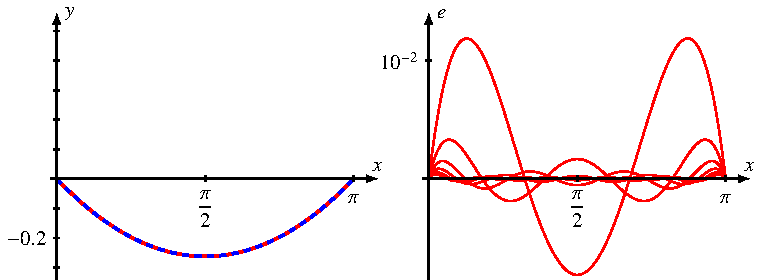
\includegraphics{chapters/070-direkt/images/ritzloesung.pdf}
\caption{Lösung des Refraktionsproblems mit dem Ritzverfahren.
Die numerische Lösung mit dem Ritz-Verfahren (rot) ist visuell nicht von
der Lösung der Euler-Lagrange-Differentialgleichung zu unterscheiden.
Der Unterschied $y_n(x)-y_\infty(x)$ ist rechts hundertfach überhöht
dargestellt.
Mit nur sechs Termen findet das Ritz-Verfahren eine Lösung mit einem
Fehler $<10^{-3}$.
\label{buch:direkt:ritz:fig:ritzloesung}}
\end{figure}


\begin{table}
\def\dglsol{
	({0.0000*\dx},{0.0000*\dy})
	-- ({0.0317*\dx},{-0.0106*\dy})
	-- ({0.0635*\dx},{-0.0210*\dy})
	-- ({0.0952*\dx},{-0.0311*\dy})
	-- ({0.1269*\dx},{-0.0411*\dy})
	-- ({0.1587*\dx},{-0.0508*\dy})
	-- ({0.1904*\dx},{-0.0603*\dy})
	-- ({0.2221*\dx},{-0.0695*\dy})
	-- ({0.2539*\dx},{-0.0786*\dy})
	-- ({0.2856*\dx},{-0.0874*\dy})
	-- ({0.3173*\dx},{-0.0960*\dy})
	-- ({0.3491*\dx},{-0.1044*\dy})
	-- ({0.3808*\dx},{-0.1126*\dy})
	-- ({0.4125*\dx},{-0.1205*\dy})
	-- ({0.4443*\dx},{-0.1282*\dy})
	-- ({0.4760*\dx},{-0.1358*\dy})
	-- ({0.5077*\dx},{-0.1430*\dy})
	-- ({0.5395*\dx},{-0.1501*\dy})
	-- ({0.5712*\dx},{-0.1570*\dy})
	-- ({0.6029*\dx},{-0.1636*\dy})
	-- ({0.6347*\dx},{-0.1700*\dy})
	-- ({0.6664*\dx},{-0.1762*\dy})
	-- ({0.6981*\dx},{-0.1822*\dy})
	-- ({0.7299*\dx},{-0.1880*\dy})
	-- ({0.7616*\dx},{-0.1935*\dy})
	-- ({0.7933*\dx},{-0.1989*\dy})
	-- ({0.8251*\dx},{-0.2040*\dy})
	-- ({0.8568*\dx},{-0.2089*\dy})
	-- ({0.8885*\dx},{-0.2136*\dy})
	-- ({0.9203*\dx},{-0.2181*\dy})
	-- ({0.9520*\dx},{-0.2224*\dy})
	-- ({0.9837*\dx},{-0.2264*\dy})
	-- ({1.0155*\dx},{-0.2302*\dy})
	-- ({1.0472*\dx},{-0.2339*\dy})
	-- ({1.0789*\dx},{-0.2373*\dy})
	-- ({1.1107*\dx},{-0.2405*\dy})
	-- ({1.1424*\dx},{-0.2434*\dy})
	-- ({1.1741*\dx},{-0.2462*\dy})
	-- ({1.2059*\dx},{-0.2488*\dy})
	-- ({1.2376*\dx},{-0.2511*\dy})
	-- ({1.2693*\dx},{-0.2532*\dy})
	-- ({1.3011*\dx},{-0.2551*\dy})
	-- ({1.3328*\dx},{-0.2568*\dy})
	-- ({1.3645*\dx},{-0.2583*\dy})
	-- ({1.3963*\dx},{-0.2596*\dy})
	-- ({1.4280*\dx},{-0.2607*\dy})
	-- ({1.4597*\dx},{-0.2615*\dy})
	-- ({1.4915*\dx},{-0.2622*\dy})
	-- ({1.5232*\dx},{-0.2626*\dy})
	-- ({1.5549*\dx},{-0.2628*\dy})
	-- ({1.5867*\dx},{-0.2628*\dy})
	-- ({1.6184*\dx},{-0.2626*\dy})
	-- ({1.6501*\dx},{-0.2622*\dy})
	-- ({1.6819*\dx},{-0.2615*\dy})
	-- ({1.7136*\dx},{-0.2607*\dy})
	-- ({1.7453*\dx},{-0.2596*\dy})
	-- ({1.7771*\dx},{-0.2583*\dy})
	-- ({1.8088*\dx},{-0.2568*\dy})
	-- ({1.8405*\dx},{-0.2551*\dy})
	-- ({1.8723*\dx},{-0.2532*\dy})
	-- ({1.9040*\dx},{-0.2511*\dy})
	-- ({1.9357*\dx},{-0.2488*\dy})
	-- ({1.9675*\dx},{-0.2462*\dy})
	-- ({1.9992*\dx},{-0.2434*\dy})
	-- ({2.0309*\dx},{-0.2405*\dy})
	-- ({2.0627*\dx},{-0.2373*\dy})
	-- ({2.0944*\dx},{-0.2339*\dy})
	-- ({2.1261*\dx},{-0.2302*\dy})
	-- ({2.1579*\dx},{-0.2264*\dy})
	-- ({2.1896*\dx},{-0.2224*\dy})
	-- ({2.2213*\dx},{-0.2181*\dy})
	-- ({2.2531*\dx},{-0.2136*\dy})
	-- ({2.2848*\dx},{-0.2089*\dy})
	-- ({2.3165*\dx},{-0.2040*\dy})
	-- ({2.3483*\dx},{-0.1989*\dy})
	-- ({2.3800*\dx},{-0.1935*\dy})
	-- ({2.4117*\dx},{-0.1880*\dy})
	-- ({2.4435*\dx},{-0.1822*\dy})
	-- ({2.4752*\dx},{-0.1762*\dy})
	-- ({2.5069*\dx},{-0.1700*\dy})
	-- ({2.5387*\dx},{-0.1636*\dy})
	-- ({2.5704*\dx},{-0.1570*\dy})
	-- ({2.6021*\dx},{-0.1501*\dy})
	-- ({2.6339*\dx},{-0.1430*\dy})
	-- ({2.6656*\dx},{-0.1358*\dy})
	-- ({2.6973*\dx},{-0.1282*\dy})
	-- ({2.7291*\dx},{-0.1205*\dy})
	-- ({2.7608*\dx},{-0.1126*\dy})
	-- ({2.7925*\dx},{-0.1044*\dy})
	-- ({2.8243*\dx},{-0.0960*\dy})
	-- ({2.8560*\dx},{-0.0874*\dy})
	-- ({2.8877*\dx},{-0.0786*\dy})
	-- ({2.9195*\dx},{-0.0695*\dy})
	-- ({2.9512*\dx},{-0.0603*\dy})
	-- ({2.9829*\dx},{-0.0508*\dy})
	-- ({3.0147*\dx},{-0.0411*\dy})
	-- ({3.0464*\dx},{-0.0311*\dy})
	-- ({3.0781*\dx},{-0.0210*\dy})
	-- ({3.1099*\dx},{-0.0106*\dy})
	-- ({3.1416*\dx},{-0.0000*\dy})
}
\def\lone{
	({0.00000*\dx},{0.00000*\dy})
	-- ({0.03173*\dx},{-0.00860*\dy})
	-- ({0.06347*\dx},{-0.01719*\dy})
	-- ({0.09520*\dx},{-0.02576*\dy})
	-- ({0.12693*\dx},{-0.03430*\dy})
	-- ({0.15867*\dx},{-0.04281*\dy})
	-- ({0.19040*\dx},{-0.05128*\dy})
	-- ({0.22213*\dx},{-0.05970*\dy})
	-- ({0.25387*\dx},{-0.06805*\dy})
	-- ({0.28560*\dx},{-0.07634*\dy})
	-- ({0.31733*\dx},{-0.08455*\dy})
	-- ({0.34907*\dx},{-0.09268*\dy})
	-- ({0.38080*\dx},{-0.10071*\dy})
	-- ({0.41253*\dx},{-0.10864*\dy})
	-- ({0.44427*\dx},{-0.11646*\dy})
	-- ({0.47600*\dx},{-0.12416*\dy})
	-- ({0.50773*\dx},{-0.13174*\dy})
	-- ({0.53947*\dx},{-0.13919*\dy})
	-- ({0.57120*\dx},{-0.14650*\dy})
	-- ({0.60293*\dx},{-0.15365*\dy})
	-- ({0.63467*\dx},{-0.16066*\dy})
	-- ({0.66640*\dx},{-0.16750*\dy})
	-- ({0.69813*\dx},{-0.17417*\dy})
	-- ({0.72986*\dx},{-0.18067*\dy})
	-- ({0.76160*\dx},{-0.18699*\dy})
	-- ({0.79333*\dx},{-0.19312*\dy})
	-- ({0.82506*\dx},{-0.19905*\dy})
	-- ({0.85680*\dx},{-0.20478*\dy})
	-- ({0.88853*\dx},{-0.21031*\dy})
	-- ({0.92026*\dx},{-0.21562*\dy})
	-- ({0.95200*\dx},{-0.22072*\dy})
	-- ({0.98373*\dx},{-0.22560*\dy})
	-- ({1.01546*\dx},{-0.23025*\dy})
	-- ({1.04720*\dx},{-0.23466*\dy})
	-- ({1.07893*\dx},{-0.23884*\dy})
	-- ({1.11066*\dx},{-0.24278*\dy})
	-- ({1.14240*\dx},{-0.24648*\dy})
	-- ({1.17413*\dx},{-0.24993*\dy})
	-- ({1.20586*\dx},{-0.25312*\dy})
	-- ({1.23760*\dx},{-0.25606*\dy})
	-- ({1.26933*\dx},{-0.25875*\dy})
	-- ({1.30106*\dx},{-0.26117*\dy})
	-- ({1.33280*\dx},{-0.26333*\dy})
	-- ({1.36453*\dx},{-0.26522*\dy})
	-- ({1.39626*\dx},{-0.26685*\dy})
	-- ({1.42800*\dx},{-0.26821*\dy})
	-- ({1.45973*\dx},{-0.26930*\dy})
	-- ({1.49146*\dx},{-0.27011*\dy})
	-- ({1.52320*\dx},{-0.27066*\dy})
	-- ({1.55493*\dx},{-0.27093*\dy})
	-- ({1.58666*\dx},{-0.27093*\dy})
	-- ({1.61840*\dx},{-0.27066*\dy})
	-- ({1.65013*\dx},{-0.27011*\dy})
	-- ({1.68186*\dx},{-0.26930*\dy})
	-- ({1.71360*\dx},{-0.26821*\dy})
	-- ({1.74533*\dx},{-0.26685*\dy})
	-- ({1.77706*\dx},{-0.26522*\dy})
	-- ({1.80880*\dx},{-0.26333*\dy})
	-- ({1.84053*\dx},{-0.26117*\dy})
	-- ({1.87226*\dx},{-0.25875*\dy})
	-- ({1.90400*\dx},{-0.25606*\dy})
	-- ({1.93573*\dx},{-0.25312*\dy})
	-- ({1.96746*\dx},{-0.24993*\dy})
	-- ({1.99920*\dx},{-0.24648*\dy})
	-- ({2.03093*\dx},{-0.24278*\dy})
	-- ({2.06266*\dx},{-0.23884*\dy})
	-- ({2.09440*\dx},{-0.23466*\dy})
	-- ({2.12613*\dx},{-0.23025*\dy})
	-- ({2.15786*\dx},{-0.22560*\dy})
	-- ({2.18959*\dx},{-0.22072*\dy})
	-- ({2.22133*\dx},{-0.21562*\dy})
	-- ({2.25306*\dx},{-0.21031*\dy})
	-- ({2.28479*\dx},{-0.20478*\dy})
	-- ({2.31653*\dx},{-0.19905*\dy})
	-- ({2.34826*\dx},{-0.19312*\dy})
	-- ({2.37999*\dx},{-0.18699*\dy})
	-- ({2.41173*\dx},{-0.18067*\dy})
	-- ({2.44346*\dx},{-0.17417*\dy})
	-- ({2.47519*\dx},{-0.16750*\dy})
	-- ({2.50693*\dx},{-0.16066*\dy})
	-- ({2.53866*\dx},{-0.15365*\dy})
	-- ({2.57039*\dx},{-0.14650*\dy})
	-- ({2.60213*\dx},{-0.13919*\dy})
	-- ({2.63386*\dx},{-0.13174*\dy})
	-- ({2.66559*\dx},{-0.12416*\dy})
	-- ({2.69733*\dx},{-0.11646*\dy})
	-- ({2.72906*\dx},{-0.10864*\dy})
	-- ({2.76079*\dx},{-0.10071*\dy})
	-- ({2.79253*\dx},{-0.09268*\dy})
	-- ({2.82426*\dx},{-0.08455*\dy})
	-- ({2.85599*\dx},{-0.07634*\dy})
	-- ({2.88773*\dx},{-0.06805*\dy})
	-- ({2.91946*\dx},{-0.05970*\dy})
	-- ({2.95119*\dx},{-0.05128*\dy})
	-- ({2.98293*\dx},{-0.04281*\dy})
	-- ({3.01466*\dx},{-0.03430*\dy})
	-- ({3.04639*\dx},{-0.02576*\dy})
	-- ({3.07813*\dx},{-0.01719*\dy})
	-- ({3.10986*\dx},{-0.00860*\dy})
	-- ({3.14159*\dx},{-0.00000*\dy})
}
\def\eone{
	({0.00000*\dx},{0.0000*\dy})
	-- ({0.03173*\dx},{0.20070*\dy})
	-- ({0.06347*\dx},{0.37988*\dy})
	-- ({0.09520*\dx},{0.53844*\dy})
	-- ({0.12693*\dx},{0.67731*\dy})
	-- ({0.15867*\dx},{0.79737*\dy})
	-- ({0.19040*\dx},{0.89953*\dy})
	-- ({0.22213*\dx},{0.98469*\dy})
	-- ({0.25387*\dx},{1.05374*\dy})
	-- ({0.28560*\dx},{1.10756*\dy})
	-- ({0.31733*\dx},{1.14702*\dy})
	-- ({0.34907*\dx},{1.17298*\dy})
	-- ({0.38080*\dx},{1.18631*\dy})
	-- ({0.41253*\dx},{1.18785*\dy})
	-- ({0.44427*\dx},{1.17843*\dy})
	-- ({0.47600*\dx},{1.15888*\dy})
	-- ({0.50773*\dx},{1.13000*\dy})
	-- ({0.53947*\dx},{1.09259*\dy})
	-- ({0.57120*\dx},{1.04743*\dy})
	-- ({0.60293*\dx},{0.99529*\dy})
	-- ({0.63467*\dx},{0.93692*\dy})
	-- ({0.66640*\dx},{0.87306*\dy})
	-- ({0.69813*\dx},{0.80441*\dy})
	-- ({0.72986*\dx},{0.73168*\dy})
	-- ({0.76160*\dx},{0.65555*\dy})
	-- ({0.79333*\dx},{0.57668*\dy})
	-- ({0.82506*\dx},{0.49571*\dy})
	-- ({0.85680*\dx},{0.41326*\dy})
	-- ({0.88853*\dx},{0.32994*\dy})
	-- ({0.92026*\dx},{0.24631*\dy})
	-- ({0.95200*\dx},{0.16293*\dy})
	-- ({0.98373*\dx},{0.08034*\dy})
	-- ({1.01546*\dx},{-0.00096*\dy})
	-- ({1.04720*\dx},{-0.08047*\dy})
	-- ({1.07893*\dx},{-0.15775*\dy})
	-- ({1.11066*\dx},{-0.23234*\dy})
	-- ({1.14240*\dx},{-0.30385*\dy})
	-- ({1.17413*\dx},{-0.37189*\dy})
	-- ({1.20586*\dx},{-0.43609*\dy})
	-- ({1.23760*\dx},{-0.49612*\dy})
	-- ({1.26933*\dx},{-0.55168*\dy})
	-- ({1.30106*\dx},{-0.60249*\dy})
	-- ({1.33280*\dx},{-0.64829*\dy})
	-- ({1.36453*\dx},{-0.68887*\dy})
	-- ({1.39626*\dx},{-0.72401*\dy})
	-- ({1.42800*\dx},{-0.75356*\dy})
	-- ({1.45973*\dx},{-0.77736*\dy})
	-- ({1.49146*\dx},{-0.79532*\dy})
	-- ({1.52320*\dx},{-0.80734*\dy})
	-- ({1.55493*\dx},{-0.81336*\dy})
	-- ({1.58666*\dx},{-0.81336*\dy})
	-- ({1.61840*\dx},{-0.80734*\dy})
	-- ({1.65013*\dx},{-0.79532*\dy})
	-- ({1.68186*\dx},{-0.77736*\dy})
	-- ({1.71360*\dx},{-0.75355*\dy})
	-- ({1.74533*\dx},{-0.72401*\dy})
	-- ({1.77706*\dx},{-0.68886*\dy})
	-- ({1.80880*\dx},{-0.64829*\dy})
	-- ({1.84053*\dx},{-0.60249*\dy})
	-- ({1.87226*\dx},{-0.55168*\dy})
	-- ({1.90400*\dx},{-0.49612*\dy})
	-- ({1.93573*\dx},{-0.43608*\dy})
	-- ({1.96746*\dx},{-0.37188*\dy})
	-- ({1.99920*\dx},{-0.30384*\dy})
	-- ({2.03093*\dx},{-0.23233*\dy})
	-- ({2.06266*\dx},{-0.15774*\dy})
	-- ({2.09440*\dx},{-0.08046*\dy})
	-- ({2.12613*\dx},{-0.00095*\dy})
	-- ({2.15786*\dx},{0.08035*\dy})
	-- ({2.18959*\dx},{0.16294*\dy})
	-- ({2.22133*\dx},{0.24632*\dy})
	-- ({2.25306*\dx},{0.32995*\dy})
	-- ({2.28479*\dx},{0.41328*\dy})
	-- ({2.31653*\dx},{0.49573*\dy})
	-- ({2.34826*\dx},{0.57670*\dy})
	-- ({2.37999*\dx},{0.65557*\dy})
	-- ({2.41173*\dx},{0.73170*\dy})
	-- ({2.44346*\dx},{0.80443*\dy})
	-- ({2.47519*\dx},{0.87307*\dy})
	-- ({2.50693*\dx},{0.93694*\dy})
	-- ({2.53866*\dx},{0.99531*\dy})
	-- ({2.57039*\dx},{1.04745*\dy})
	-- ({2.60213*\dx},{1.09261*\dy})
	-- ({2.63386*\dx},{1.13002*\dy})
	-- ({2.66559*\dx},{1.15890*\dy})
	-- ({2.69733*\dx},{1.17845*\dy})
	-- ({2.72906*\dx},{1.18787*\dy})
	-- ({2.76079*\dx},{1.18634*\dy})
	-- ({2.79253*\dx},{1.17301*\dy})
	-- ({2.82426*\dx},{1.14704*\dy})
	-- ({2.85599*\dx},{1.10758*\dy})
	-- ({2.88773*\dx},{1.05377*\dy})
	-- ({2.91946*\dx},{0.98472*\dy})
	-- ({2.95119*\dx},{0.89956*\dy})
	-- ({2.98293*\dx},{0.79739*\dy})
	-- ({3.01466*\dx},{0.67733*\dy})
	-- ({3.04639*\dx},{0.53847*\dy})
	-- ({3.07813*\dx},{0.37991*\dy})
	-- ({3.10986*\dx},{0.20073*\dy})
	-- ({3.14159*\dx},{0.00003*\dy})
}
\def\ltwo{
	({0.00000*\dx},{0.00000*\dy})
	-- ({0.03173*\dx},{-0.00960*\dy})
	-- ({0.06347*\dx},{-0.01918*\dy})
	-- ({0.09520*\dx},{-0.02873*\dy})
	-- ({0.12693*\dx},{-0.03822*\dy})
	-- ({0.15867*\dx},{-0.04765*\dy})
	-- ({0.19040*\dx},{-0.05699*\dy})
	-- ({0.22213*\dx},{-0.06622*\dy})
	-- ({0.25387*\dx},{-0.07534*\dy})
	-- ({0.28560*\dx},{-0.08433*\dy})
	-- ({0.31733*\dx},{-0.09316*\dy})
	-- ({0.34907*\dx},{-0.10184*\dy})
	-- ({0.38080*\dx},{-0.11034*\dy})
	-- ({0.41253*\dx},{-0.11865*\dy})
	-- ({0.44427*\dx},{-0.12677*\dy})
	-- ({0.47600*\dx},{-0.13468*\dy})
	-- ({0.50773*\dx},{-0.14236*\dy})
	-- ({0.53947*\dx},{-0.14982*\dy})
	-- ({0.57120*\dx},{-0.15705*\dy})
	-- ({0.60293*\dx},{-0.16404*\dy})
	-- ({0.63467*\dx},{-0.17078*\dy})
	-- ({0.66640*\dx},{-0.17727*\dy})
	-- ({0.69813*\dx},{-0.18350*\dy})
	-- ({0.72986*\dx},{-0.18948*\dy})
	-- ({0.76160*\dx},{-0.19520*\dy})
	-- ({0.79333*\dx},{-0.20066*\dy})
	-- ({0.82506*\dx},{-0.20586*\dy})
	-- ({0.85680*\dx},{-0.21080*\dy})
	-- ({0.88853*\dx},{-0.21549*\dy})
	-- ({0.92026*\dx},{-0.21992*\dy})
	-- ({0.95200*\dx},{-0.22409*\dy})
	-- ({0.98373*\dx},{-0.22802*\dy})
	-- ({1.01546*\dx},{-0.23170*\dy})
	-- ({1.04720*\dx},{-0.23514*\dy})
	-- ({1.07893*\dx},{-0.23835*\dy})
	-- ({1.11066*\dx},{-0.24132*\dy})
	-- ({1.14240*\dx},{-0.24406*\dy})
	-- ({1.17413*\dx},{-0.24659*\dy})
	-- ({1.20586*\dx},{-0.24889*\dy})
	-- ({1.23760*\dx},{-0.25098*\dy})
	-- ({1.26933*\dx},{-0.25287*\dy})
	-- ({1.30106*\dx},{-0.25455*\dy})
	-- ({1.33280*\dx},{-0.25603*\dy})
	-- ({1.36453*\dx},{-0.25732*\dy})
	-- ({1.39626*\dx},{-0.25842*\dy})
	-- ({1.42800*\dx},{-0.25933*\dy})
	-- ({1.45973*\dx},{-0.26005*\dy})
	-- ({1.49146*\dx},{-0.26060*\dy})
	-- ({1.52320*\dx},{-0.26096*\dy})
	-- ({1.55493*\dx},{-0.26114*\dy})
	-- ({1.58666*\dx},{-0.26114*\dy})
	-- ({1.61840*\dx},{-0.26096*\dy})
	-- ({1.65013*\dx},{-0.26060*\dy})
	-- ({1.68186*\dx},{-0.26005*\dy})
	-- ({1.71360*\dx},{-0.25933*\dy})
	-- ({1.74533*\dx},{-0.25842*\dy})
	-- ({1.77706*\dx},{-0.25732*\dy})
	-- ({1.80880*\dx},{-0.25603*\dy})
	-- ({1.84053*\dx},{-0.25455*\dy})
	-- ({1.87226*\dx},{-0.25287*\dy})
	-- ({1.90400*\dx},{-0.25098*\dy})
	-- ({1.93573*\dx},{-0.24889*\dy})
	-- ({1.96746*\dx},{-0.24659*\dy})
	-- ({1.99920*\dx},{-0.24406*\dy})
	-- ({2.03093*\dx},{-0.24132*\dy})
	-- ({2.06266*\dx},{-0.23835*\dy})
	-- ({2.09440*\dx},{-0.23514*\dy})
	-- ({2.12613*\dx},{-0.23170*\dy})
	-- ({2.15786*\dx},{-0.22802*\dy})
	-- ({2.18959*\dx},{-0.22409*\dy})
	-- ({2.22133*\dx},{-0.21992*\dy})
	-- ({2.25306*\dx},{-0.21549*\dy})
	-- ({2.28479*\dx},{-0.21080*\dy})
	-- ({2.31653*\dx},{-0.20586*\dy})
	-- ({2.34826*\dx},{-0.20066*\dy})
	-- ({2.37999*\dx},{-0.19520*\dy})
	-- ({2.41173*\dx},{-0.18948*\dy})
	-- ({2.44346*\dx},{-0.18350*\dy})
	-- ({2.47519*\dx},{-0.17727*\dy})
	-- ({2.50693*\dx},{-0.17078*\dy})
	-- ({2.53866*\dx},{-0.16404*\dy})
	-- ({2.57039*\dx},{-0.15705*\dy})
	-- ({2.60213*\dx},{-0.14982*\dy})
	-- ({2.63386*\dx},{-0.14236*\dy})
	-- ({2.66559*\dx},{-0.13468*\dy})
	-- ({2.69733*\dx},{-0.12677*\dy})
	-- ({2.72906*\dx},{-0.11865*\dy})
	-- ({2.76079*\dx},{-0.11034*\dy})
	-- ({2.79253*\dx},{-0.10184*\dy})
	-- ({2.82426*\dx},{-0.09316*\dy})
	-- ({2.85599*\dx},{-0.08433*\dy})
	-- ({2.88773*\dx},{-0.07534*\dy})
	-- ({2.91946*\dx},{-0.06622*\dy})
	-- ({2.95119*\dx},{-0.05699*\dy})
	-- ({2.98293*\dx},{-0.04765*\dy})
	-- ({3.01466*\dx},{-0.03822*\dy})
	-- ({3.04639*\dx},{-0.02873*\dy})
	-- ({3.07813*\dx},{-0.01918*\dy})
	-- ({3.10986*\dx},{-0.00960*\dy})
	-- ({3.14159*\dx},{-0.00000*\dy})
}
\def\etwo{
	({0.00000*\dx},{0.0000*\dy})
	-- ({0.03173*\dx},{0.10044*\dy})
	-- ({0.06347*\dx},{0.18025*\dy})
	-- ({0.09520*\dx},{0.24122*\dy})
	-- ({0.12693*\dx},{0.28514*\dy})
	-- ({0.15867*\dx},{0.31376*\dy})
	-- ({0.19040*\dx},{0.32879*\dy})
	-- ({0.22213*\dx},{0.33190*\dy})
	-- ({0.25387*\dx},{0.32471*\dy})
	-- ({0.28560*\dx},{0.30877*\dy})
	-- ({0.31733*\dx},{0.28559*\dy})
	-- ({0.34907*\dx},{0.25658*\dy})
	-- ({0.38080*\dx},{0.22308*\dy})
	-- ({0.41253*\dx},{0.18634*\dy})
	-- ({0.44427*\dx},{0.14754*\dy})
	-- ({0.47600*\dx},{0.10775*\dy})
	-- ({0.50773*\dx},{0.06794*\dy})
	-- ({0.53947*\dx},{0.02901*\dy})
	-- ({0.57120*\dx},{-0.00827*\dy})
	-- ({0.60293*\dx},{-0.04321*\dy})
	-- ({0.63467*\dx},{-0.07523*\dy})
	-- ({0.66640*\dx},{-0.10384*\dy})
	-- ({0.69813*\dx},{-0.12867*\dy})
	-- ({0.72986*\dx},{-0.14941*\dy})
	-- ({0.76160*\dx},{-0.16587*\dy})
	-- ({0.79333*\dx},{-0.17794*\dy})
	-- ({0.82506*\dx},{-0.18560*\dy})
	-- ({0.85680*\dx},{-0.18889*\dy})
	-- ({0.88853*\dx},{-0.18794*\dy})
	-- ({0.92026*\dx},{-0.18296*\dy})
	-- ({0.95200*\dx},{-0.17419*\dy})
	-- ({0.98373*\dx},{-0.16194*\dy})
	-- ({1.01546*\dx},{-0.14657*\dy})
	-- ({1.04720*\dx},{-0.12849*\dy})
	-- ({1.07893*\dx},{-0.10811*\dy})
	-- ({1.11066*\dx},{-0.08590*\dy})
	-- ({1.14240*\dx},{-0.06233*\dy})
	-- ({1.17413*\dx},{-0.03788*\dy})
	-- ({1.20586*\dx},{-0.01303*\dy})
	-- ({1.23760*\dx},{0.01173*\dy})
	-- ({1.26933*\dx},{0.03595*\dy})
	-- ({1.30106*\dx},{0.05918*\dy})
	-- ({1.33280*\dx},{0.08099*\dy})
	-- ({1.36453*\dx},{0.10099*\dy})
	-- ({1.39626*\dx},{0.11883*\dy})
	-- ({1.42800*\dx},{0.13419*\dy})
	-- ({1.45973*\dx},{0.14681*\dy})
	-- ({1.49146*\dx},{0.15647*\dy})
	-- ({1.52320*\dx},{0.16301*\dy})
	-- ({1.55493*\dx},{0.16630*\dy})
	-- ({1.58666*\dx},{0.16630*\dy})
	-- ({1.61840*\dx},{0.16301*\dy})
	-- ({1.65013*\dx},{0.15647*\dy})
	-- ({1.68186*\dx},{0.14681*\dy})
	-- ({1.71360*\dx},{0.13419*\dy})
	-- ({1.74533*\dx},{0.11883*\dy})
	-- ({1.77706*\dx},{0.10099*\dy})
	-- ({1.80880*\dx},{0.08099*\dy})
	-- ({1.84053*\dx},{0.05918*\dy})
	-- ({1.87226*\dx},{0.03596*\dy})
	-- ({1.90400*\dx},{0.01174*\dy})
	-- ({1.93573*\dx},{-0.01303*\dy})
	-- ({1.96746*\dx},{-0.03787*\dy})
	-- ({1.99920*\dx},{-0.06233*\dy})
	-- ({2.03093*\dx},{-0.08590*\dy})
	-- ({2.06266*\dx},{-0.10810*\dy})
	-- ({2.09440*\dx},{-0.12848*\dy})
	-- ({2.12613*\dx},{-0.14656*\dy})
	-- ({2.15786*\dx},{-0.16193*\dy})
	-- ({2.18959*\dx},{-0.17417*\dy})
	-- ({2.22133*\dx},{-0.18294*\dy})
	-- ({2.25306*\dx},{-0.18793*\dy})
	-- ({2.28479*\dx},{-0.18888*\dy})
	-- ({2.31653*\dx},{-0.18558*\dy})
	-- ({2.34826*\dx},{-0.17793*\dy})
	-- ({2.37999*\dx},{-0.16586*\dy})
	-- ({2.41173*\dx},{-0.14939*\dy})
	-- ({2.44346*\dx},{-0.12865*\dy})
	-- ({2.47519*\dx},{-0.10383*\dy})
	-- ({2.50693*\dx},{-0.07521*\dy})
	-- ({2.53866*\dx},{-0.04319*\dy})
	-- ({2.57039*\dx},{-0.00825*\dy})
	-- ({2.60213*\dx},{0.02903*\dy})
	-- ({2.63386*\dx},{0.06796*\dy})
	-- ({2.66559*\dx},{0.10777*\dy})
	-- ({2.69733*\dx},{0.14756*\dy})
	-- ({2.72906*\dx},{0.18637*\dy})
	-- ({2.76079*\dx},{0.22310*\dy})
	-- ({2.79253*\dx},{0.25661*\dy})
	-- ({2.82426*\dx},{0.28562*\dy})
	-- ({2.85599*\dx},{0.30880*\dy})
	-- ({2.88773*\dx},{0.32473*\dy})
	-- ({2.91946*\dx},{0.33192*\dy})
	-- ({2.95119*\dx},{0.32881*\dy})
	-- ({2.98293*\dx},{0.31379*\dy})
	-- ({3.01466*\dx},{0.28517*\dy})
	-- ({3.04639*\dx},{0.24125*\dy})
	-- ({3.07813*\dx},{0.18028*\dy})
	-- ({3.10986*\dx},{0.10047*\dy})
	-- ({3.14159*\dx},{0.00003*\dy})
}
\def\lthree{
	({0.00000*\dx},{0.00000*\dy})
	-- ({0.03173*\dx},{-0.00996*\dy})
	-- ({0.06347*\dx},{-0.01990*\dy})
	-- ({0.09520*\dx},{-0.02978*\dy})
	-- ({0.12693*\dx},{-0.03958*\dy})
	-- ({0.15867*\dx},{-0.04929*\dy})
	-- ({0.19040*\dx},{-0.05886*\dy})
	-- ({0.22213*\dx},{-0.06829*\dy})
	-- ({0.25387*\dx},{-0.07754*\dy})
	-- ({0.28560*\dx},{-0.08661*\dy})
	-- ({0.31733*\dx},{-0.09548*\dy})
	-- ({0.34907*\dx},{-0.10413*\dy})
	-- ({0.38080*\dx},{-0.11254*\dy})
	-- ({0.41253*\dx},{-0.12072*\dy})
	-- ({0.44427*\dx},{-0.12864*\dy})
	-- ({0.47600*\dx},{-0.13632*\dy})
	-- ({0.50773*\dx},{-0.14373*\dy})
	-- ({0.53947*\dx},{-0.15089*\dy})
	-- ({0.57120*\dx},{-0.15779*\dy})
	-- ({0.60293*\dx},{-0.16443*\dy})
	-- ({0.63467*\dx},{-0.17081*\dy})
	-- ({0.66640*\dx},{-0.17695*\dy})
	-- ({0.69813*\dx},{-0.18284*\dy})
	-- ({0.72986*\dx},{-0.18849*\dy})
	-- ({0.76160*\dx},{-0.19391*\dy})
	-- ({0.79333*\dx},{-0.19911*\dy})
	-- ({0.82506*\dx},{-0.20408*\dy})
	-- ({0.85680*\dx},{-0.20885*\dy})
	-- ({0.88853*\dx},{-0.21341*\dy})
	-- ({0.92026*\dx},{-0.21776*\dy})
	-- ({0.95200*\dx},{-0.22192*\dy})
	-- ({0.98373*\dx},{-0.22589*\dy})
	-- ({1.01546*\dx},{-0.22966*\dy})
	-- ({1.04720*\dx},{-0.23325*\dy})
	-- ({1.07893*\dx},{-0.23665*\dy})
	-- ({1.11066*\dx},{-0.23986*\dy})
	-- ({1.14240*\dx},{-0.24288*\dy})
	-- ({1.17413*\dx},{-0.24571*\dy})
	-- ({1.20586*\dx},{-0.24834*\dy})
	-- ({1.23760*\dx},{-0.25077*\dy})
	-- ({1.26933*\dx},{-0.25301*\dy})
	-- ({1.30106*\dx},{-0.25504*\dy})
	-- ({1.33280*\dx},{-0.25685*\dy})
	-- ({1.36453*\dx},{-0.25845*\dy})
	-- ({1.39626*\dx},{-0.25984*\dy})
	-- ({1.42800*\dx},{-0.26100*\dy})
	-- ({1.45973*\dx},{-0.26193*\dy})
	-- ({1.49146*\dx},{-0.26263*\dy})
	-- ({1.52320*\dx},{-0.26310*\dy})
	-- ({1.55493*\dx},{-0.26333*\dy})
	-- ({1.58666*\dx},{-0.26333*\dy})
	-- ({1.61840*\dx},{-0.26310*\dy})
	-- ({1.65013*\dx},{-0.26263*\dy})
	-- ({1.68186*\dx},{-0.26193*\dy})
	-- ({1.71360*\dx},{-0.26100*\dy})
	-- ({1.74533*\dx},{-0.25984*\dy})
	-- ({1.77706*\dx},{-0.25845*\dy})
	-- ({1.80880*\dx},{-0.25685*\dy})
	-- ({1.84053*\dx},{-0.25504*\dy})
	-- ({1.87226*\dx},{-0.25301*\dy})
	-- ({1.90400*\dx},{-0.25077*\dy})
	-- ({1.93573*\dx},{-0.24834*\dy})
	-- ({1.96746*\dx},{-0.24571*\dy})
	-- ({1.99920*\dx},{-0.24288*\dy})
	-- ({2.03093*\dx},{-0.23986*\dy})
	-- ({2.06266*\dx},{-0.23665*\dy})
	-- ({2.09440*\dx},{-0.23325*\dy})
	-- ({2.12613*\dx},{-0.22966*\dy})
	-- ({2.15786*\dx},{-0.22589*\dy})
	-- ({2.18959*\dx},{-0.22192*\dy})
	-- ({2.22133*\dx},{-0.21776*\dy})
	-- ({2.25306*\dx},{-0.21341*\dy})
	-- ({2.28479*\dx},{-0.20885*\dy})
	-- ({2.31653*\dx},{-0.20408*\dy})
	-- ({2.34826*\dx},{-0.19911*\dy})
	-- ({2.37999*\dx},{-0.19391*\dy})
	-- ({2.41173*\dx},{-0.18849*\dy})
	-- ({2.44346*\dx},{-0.18284*\dy})
	-- ({2.47519*\dx},{-0.17695*\dy})
	-- ({2.50693*\dx},{-0.17081*\dy})
	-- ({2.53866*\dx},{-0.16443*\dy})
	-- ({2.57039*\dx},{-0.15779*\dy})
	-- ({2.60213*\dx},{-0.15089*\dy})
	-- ({2.63386*\dx},{-0.14373*\dy})
	-- ({2.66559*\dx},{-0.13632*\dy})
	-- ({2.69733*\dx},{-0.12864*\dy})
	-- ({2.72906*\dx},{-0.12072*\dy})
	-- ({2.76079*\dx},{-0.11254*\dy})
	-- ({2.79253*\dx},{-0.10413*\dy})
	-- ({2.82426*\dx},{-0.09548*\dy})
	-- ({2.85599*\dx},{-0.08661*\dy})
	-- ({2.88773*\dx},{-0.07754*\dy})
	-- ({2.91946*\dx},{-0.06829*\dy})
	-- ({2.95119*\dx},{-0.05886*\dy})
	-- ({2.98293*\dx},{-0.04929*\dy})
	-- ({3.01466*\dx},{-0.03958*\dy})
	-- ({3.04639*\dx},{-0.02978*\dy})
	-- ({3.07813*\dx},{-0.01990*\dy})
	-- ({3.10986*\dx},{-0.00996*\dy})
	-- ({3.14159*\dx},{-0.00000*\dy})
}
\def\ethree{
	({0.00000*\dx},{0.0000*\dy})
	-- ({0.03173*\dx},{0.06423*\dy})
	-- ({0.06347*\dx},{0.10871*\dy})
	-- ({0.09520*\dx},{0.13613*\dy})
	-- ({0.12693*\dx},{0.14909*\dy})
	-- ({0.15867*\dx},{0.15011*\dy})
	-- ({0.19040*\dx},{0.14157*\dy})
	-- ({0.22213*\dx},{0.12572*\dy})
	-- ({0.25387*\dx},{0.10465*\dy})
	-- ({0.28560*\dx},{0.08025*\dy})
	-- ({0.31733*\dx},{0.05422*\dy})
	-- ({0.34907*\dx},{0.02803*\dy})
	-- ({0.38080*\dx},{0.00294*\dy})
	-- ({0.41253*\dx},{-0.02001*\dy})
	-- ({0.44427*\dx},{-0.04001*\dy})
	-- ({0.47600*\dx},{-0.05646*\dy})
	-- ({0.50773*\dx},{-0.06897*\dy})
	-- ({0.53947*\dx},{-0.07735*\dy})
	-- ({0.57120*\dx},{-0.08159*\dy})
	-- ({0.60293*\dx},{-0.08184*\dy})
	-- ({0.63467*\dx},{-0.07838*\dy})
	-- ({0.66640*\dx},{-0.07163*\dy})
	-- ({0.69813*\dx},{-0.06208*\dy})
	-- ({0.72986*\dx},{-0.05031*\dy})
	-- ({0.76160*\dx},{-0.03692*\dy})
	-- ({0.79333*\dx},{-0.02256*\dy})
	-- ({0.82506*\dx},{-0.00786*\dy})
	-- ({0.85680*\dx},{0.00658*\dy})
	-- ({0.88853*\dx},{0.02020*\dy})
	-- ({0.92026*\dx},{0.03247*\dy})
	-- ({0.95200*\dx},{0.04299*\dy})
	-- ({0.98373*\dx},{0.05139*\dy})
	-- ({1.01546*\dx},{0.05743*\dy})
	-- ({1.04720*\dx},{0.06095*\dy})
	-- ({1.07893*\dx},{0.06191*\dy})
	-- ({1.11066*\dx},{0.06034*\dy})
	-- ({1.14240*\dx},{0.05638*\dy})
	-- ({1.17413*\dx},{0.05025*\dy})
	-- ({1.20586*\dx},{0.04224*\dy})
	-- ({1.23760*\dx},{0.03271*\dy})
	-- ({1.26933*\dx},{0.02207*\dy})
	-- ({1.30106*\dx},{0.01075*\dy})
	-- ({1.33280*\dx},{-0.00080*\dy})
	-- ({1.36453*\dx},{-0.01212*\dy})
	-- ({1.39626*\dx},{-0.02276*\dy})
	-- ({1.42800*\dx},{-0.03233*\dy})
	-- ({1.45973*\dx},{-0.04046*\dy})
	-- ({1.49146*\dx},{-0.04683*\dy})
	-- ({1.52320*\dx},{-0.05122*\dy})
	-- ({1.55493*\dx},{-0.05346*\dy})
	-- ({1.58666*\dx},{-0.05346*\dy})
	-- ({1.61840*\dx},{-0.05122*\dy})
	-- ({1.65013*\dx},{-0.04683*\dy})
	-- ({1.68186*\dx},{-0.04045*\dy})
	-- ({1.71360*\dx},{-0.03233*\dy})
	-- ({1.74533*\dx},{-0.02276*\dy})
	-- ({1.77706*\dx},{-0.01211*\dy})
	-- ({1.80880*\dx},{-0.00080*\dy})
	-- ({1.84053*\dx},{0.01075*\dy})
	-- ({1.87226*\dx},{0.02207*\dy})
	-- ({1.90400*\dx},{0.03272*\dy})
	-- ({1.93573*\dx},{0.04225*\dy})
	-- ({1.96746*\dx},{0.05025*\dy})
	-- ({1.99920*\dx},{0.05639*\dy})
	-- ({2.03093*\dx},{0.06035*\dy})
	-- ({2.06266*\dx},{0.06192*\dy})
	-- ({2.09440*\dx},{0.06096*\dy})
	-- ({2.12613*\dx},{0.05744*\dy})
	-- ({2.15786*\dx},{0.05140*\dy})
	-- ({2.18959*\dx},{0.04300*\dy})
	-- ({2.22133*\dx},{0.03249*\dy})
	-- ({2.25306*\dx},{0.02021*\dy})
	-- ({2.28479*\dx},{0.00660*\dy})
	-- ({2.31653*\dx},{-0.00784*\dy})
	-- ({2.34826*\dx},{-0.02255*\dy})
	-- ({2.37999*\dx},{-0.03691*\dy})
	-- ({2.41173*\dx},{-0.05029*\dy})
	-- ({2.44346*\dx},{-0.06206*\dy})
	-- ({2.47519*\dx},{-0.07161*\dy})
	-- ({2.50693*\dx},{-0.07836*\dy})
	-- ({2.53866*\dx},{-0.08182*\dy})
	-- ({2.57039*\dx},{-0.08157*\dy})
	-- ({2.60213*\dx},{-0.07733*\dy})
	-- ({2.63386*\dx},{-0.06895*\dy})
	-- ({2.66559*\dx},{-0.05643*\dy})
	-- ({2.69733*\dx},{-0.03999*\dy})
	-- ({2.72906*\dx},{-0.01999*\dy})
	-- ({2.76079*\dx},{0.00296*\dy})
	-- ({2.79253*\dx},{0.02805*\dy})
	-- ({2.82426*\dx},{0.05424*\dy})
	-- ({2.85599*\dx},{0.08028*\dy})
	-- ({2.88773*\dx},{0.10468*\dy})
	-- ({2.91946*\dx},{0.12575*\dy})
	-- ({2.95119*\dx},{0.14159*\dy})
	-- ({2.98293*\dx},{0.15013*\dy})
	-- ({3.01466*\dx},{0.14912*\dy})
	-- ({3.04639*\dx},{0.13616*\dy})
	-- ({3.07813*\dx},{0.10874*\dy})
	-- ({3.10986*\dx},{0.06425*\dy})
	-- ({3.14159*\dx},{0.00003*\dy})
}
\def\lfour{
	({0.00000*\dx},{0.00000*\dy})
	-- ({0.03173*\dx},{-0.01015*\dy})
	-- ({0.06347*\dx},{-0.02026*\dy})
	-- ({0.09520*\dx},{-0.03030*\dy})
	-- ({0.12693*\dx},{-0.04023*\dy})
	-- ({0.15867*\dx},{-0.05004*\dy})
	-- ({0.19040*\dx},{-0.05968*\dy})
	-- ({0.22213*\dx},{-0.06913*\dy})
	-- ({0.25387*\dx},{-0.07837*\dy})
	-- ({0.28560*\dx},{-0.08739*\dy})
	-- ({0.31733*\dx},{-0.09616*\dy})
	-- ({0.34907*\dx},{-0.10468*\dy})
	-- ({0.38080*\dx},{-0.11295*\dy})
	-- ({0.41253*\dx},{-0.12096*\dy})
	-- ({0.44427*\dx},{-0.12870*\dy})
	-- ({0.47600*\dx},{-0.13619*\dy})
	-- ({0.50773*\dx},{-0.14344*\dy})
	-- ({0.53947*\dx},{-0.15043*\dy})
	-- ({0.57120*\dx},{-0.15719*\dy})
	-- ({0.60293*\dx},{-0.16373*\dy})
	-- ({0.63467*\dx},{-0.17004*\dy})
	-- ({0.66640*\dx},{-0.17615*\dy})
	-- ({0.69813*\dx},{-0.18204*\dy})
	-- ({0.72986*\dx},{-0.18774*\dy})
	-- ({0.76160*\dx},{-0.19325*\dy})
	-- ({0.79333*\dx},{-0.19856*\dy})
	-- ({0.82506*\dx},{-0.20368*\dy})
	-- ({0.85680*\dx},{-0.20861*\dy})
	-- ({0.88853*\dx},{-0.21334*\dy})
	-- ({0.92026*\dx},{-0.21788*\dy})
	-- ({0.95200*\dx},{-0.22221*\dy})
	-- ({0.98373*\dx},{-0.22633*\dy})
	-- ({1.01546*\dx},{-0.23025*\dy})
	-- ({1.04720*\dx},{-0.23394*\dy})
	-- ({1.07893*\dx},{-0.23741*\dy})
	-- ({1.11066*\dx},{-0.24066*\dy})
	-- ({1.14240*\dx},{-0.24367*\dy})
	-- ({1.17413*\dx},{-0.24646*\dy})
	-- ({1.20586*\dx},{-0.24901*\dy})
	-- ({1.23760*\dx},{-0.25134*\dy})
	-- ({1.26933*\dx},{-0.25343*\dy})
	-- ({1.30106*\dx},{-0.25530*\dy})
	-- ({1.33280*\dx},{-0.25694*\dy})
	-- ({1.36453*\dx},{-0.25837*\dy})
	-- ({1.39626*\dx},{-0.25958*\dy})
	-- ({1.42800*\dx},{-0.26058*\dy})
	-- ({1.45973*\dx},{-0.26137*\dy})
	-- ({1.49146*\dx},{-0.26196*\dy})
	-- ({1.52320*\dx},{-0.26235*\dy})
	-- ({1.55493*\dx},{-0.26255*\dy})
	-- ({1.58666*\dx},{-0.26255*\dy})
	-- ({1.61840*\dx},{-0.26235*\dy})
	-- ({1.65013*\dx},{-0.26196*\dy})
	-- ({1.68186*\dx},{-0.26137*\dy})
	-- ({1.71360*\dx},{-0.26058*\dy})
	-- ({1.74533*\dx},{-0.25958*\dy})
	-- ({1.77706*\dx},{-0.25837*\dy})
	-- ({1.80880*\dx},{-0.25694*\dy})
	-- ({1.84053*\dx},{-0.25530*\dy})
	-- ({1.87226*\dx},{-0.25343*\dy})
	-- ({1.90400*\dx},{-0.25134*\dy})
	-- ({1.93573*\dx},{-0.24901*\dy})
	-- ({1.96746*\dx},{-0.24646*\dy})
	-- ({1.99920*\dx},{-0.24367*\dy})
	-- ({2.03093*\dx},{-0.24066*\dy})
	-- ({2.06266*\dx},{-0.23741*\dy})
	-- ({2.09440*\dx},{-0.23394*\dy})
	-- ({2.12613*\dx},{-0.23025*\dy})
	-- ({2.15786*\dx},{-0.22633*\dy})
	-- ({2.18959*\dx},{-0.22221*\dy})
	-- ({2.22133*\dx},{-0.21788*\dy})
	-- ({2.25306*\dx},{-0.21334*\dy})
	-- ({2.28479*\dx},{-0.20861*\dy})
	-- ({2.31653*\dx},{-0.20368*\dy})
	-- ({2.34826*\dx},{-0.19856*\dy})
	-- ({2.37999*\dx},{-0.19325*\dy})
	-- ({2.41173*\dx},{-0.18774*\dy})
	-- ({2.44346*\dx},{-0.18204*\dy})
	-- ({2.47519*\dx},{-0.17615*\dy})
	-- ({2.50693*\dx},{-0.17004*\dy})
	-- ({2.53866*\dx},{-0.16373*\dy})
	-- ({2.57039*\dx},{-0.15719*\dy})
	-- ({2.60213*\dx},{-0.15043*\dy})
	-- ({2.63386*\dx},{-0.14344*\dy})
	-- ({2.66559*\dx},{-0.13619*\dy})
	-- ({2.69733*\dx},{-0.12870*\dy})
	-- ({2.72906*\dx},{-0.12096*\dy})
	-- ({2.76079*\dx},{-0.11295*\dy})
	-- ({2.79253*\dx},{-0.10468*\dy})
	-- ({2.82426*\dx},{-0.09616*\dy})
	-- ({2.85599*\dx},{-0.08739*\dy})
	-- ({2.88773*\dx},{-0.07837*\dy})
	-- ({2.91946*\dx},{-0.06913*\dy})
	-- ({2.95119*\dx},{-0.05968*\dy})
	-- ({2.98293*\dx},{-0.05004*\dy})
	-- ({3.01466*\dx},{-0.04023*\dy})
	-- ({3.04639*\dx},{-0.03030*\dy})
	-- ({3.07813*\dx},{-0.02026*\dy})
	-- ({3.10986*\dx},{-0.01015*\dy})
	-- ({3.14159*\dx},{-0.00000*\dy})
}
\def\efour{
	({0.00000*\dx},{0.0000*\dy})
	-- ({0.03173*\dx},{0.04581*\dy})
	-- ({0.06347*\dx},{0.07276*\dy})
	-- ({0.09520*\dx},{0.08439*\dy})
	-- ({0.12693*\dx},{0.08406*\dy})
	-- ({0.15867*\dx},{0.07492*\dy})
	-- ({0.19040*\dx},{0.05986*\dy})
	-- ({0.22213*\dx},{0.04142*\dy})
	-- ({0.25387*\dx},{0.02182*\dy})
	-- ({0.28560*\dx},{0.00286*\dy})
	-- ({0.31733*\dx},{-0.01403*\dy})
	-- ({0.34907*\dx},{-0.02783*\dy})
	-- ({0.38080*\dx},{-0.03790*\dy})
	-- ({0.41253*\dx},{-0.04392*\dy})
	-- ({0.44427*\dx},{-0.04593*\dy})
	-- ({0.47600*\dx},{-0.04421*\dy})
	-- ({0.50773*\dx},{-0.03925*\dy})
	-- ({0.53947*\dx},{-0.03172*\dy})
	-- ({0.57120*\dx},{-0.02238*\dy})
	-- ({0.60293*\dx},{-0.01204*\dy})
	-- ({0.63467*\dx},{-0.00150*\dy})
	-- ({0.66640*\dx},{0.00849*\dy})
	-- ({0.69813*\dx},{0.01729*\dy})
	-- ({0.72986*\dx},{0.02437*\dy})
	-- ({0.76160*\dx},{0.02935*\dy})
	-- ({0.79333*\dx},{0.03202*\dy})
	-- ({0.82506*\dx},{0.03234*\dy})
	-- ({0.85680*\dx},{0.03041*\dy})
	-- ({0.88853*\dx},{0.02647*\dy})
	-- ({0.92026*\dx},{0.02089*\dy})
	-- ({0.95200*\dx},{0.01411*\dy})
	-- ({0.98373*\dx},{0.00666*\dy})
	-- ({1.01546*\dx},{-0.00096*\dy})
	-- ({1.04720*\dx},{-0.00821*\dy})
	-- ({1.07893*\dx},{-0.01462*\dy})
	-- ({1.11066*\dx},{-0.01979*\dy})
	-- ({1.14240*\dx},{-0.02341*\dy})
	-- ({1.17413*\dx},{-0.02529*\dy})
	-- ({1.20586*\dx},{-0.02534*\dy})
	-- ({1.23760*\dx},{-0.02360*\dy})
	-- ({1.26933*\dx},{-0.02023*\dy})
	-- ({1.30106*\dx},{-0.01549*\dy})
	-- ({1.33280*\dx},{-0.00971*\dy})
	-- ({1.36453*\dx},{-0.00331*\dy})
	-- ({1.39626*\dx},{0.00328*\dy})
	-- ({1.42800*\dx},{0.00961*\dy})
	-- ({1.45973*\dx},{0.01527*\dy})
	-- ({1.49146*\dx},{0.01987*\dy})
	-- ({1.52320*\dx},{0.02312*\dy})
	-- ({1.55493*\dx},{0.02480*\dy})
	-- ({1.58666*\dx},{0.02480*\dy})
	-- ({1.61840*\dx},{0.02312*\dy})
	-- ({1.65013*\dx},{0.01987*\dy})
	-- ({1.68186*\dx},{0.01527*\dy})
	-- ({1.71360*\dx},{0.00961*\dy})
	-- ({1.74533*\dx},{0.00328*\dy})
	-- ({1.77706*\dx},{-0.00331*\dy})
	-- ({1.80880*\dx},{-0.00971*\dy})
	-- ({1.84053*\dx},{-0.01548*\dy})
	-- ({1.87226*\dx},{-0.02022*\dy})
	-- ({1.90400*\dx},{-0.02359*\dy})
	-- ({1.93573*\dx},{-0.02533*\dy})
	-- ({1.96746*\dx},{-0.02528*\dy})
	-- ({1.99920*\dx},{-0.02340*\dy})
	-- ({2.03093*\dx},{-0.01978*\dy})
	-- ({2.06266*\dx},{-0.01461*\dy})
	-- ({2.09440*\dx},{-0.00819*\dy})
	-- ({2.12613*\dx},{-0.00094*\dy})
	-- ({2.15786*\dx},{0.00667*\dy})
	-- ({2.18959*\dx},{0.01413*\dy})
	-- ({2.22133*\dx},{0.02090*\dy})
	-- ({2.25306*\dx},{0.02648*\dy})
	-- ({2.28479*\dx},{0.03042*\dy})
	-- ({2.31653*\dx},{0.03236*\dy})
	-- ({2.34826*\dx},{0.03204*\dy})
	-- ({2.37999*\dx},{0.02937*\dy})
	-- ({2.41173*\dx},{0.02439*\dy})
	-- ({2.44346*\dx},{0.01731*\dy})
	-- ({2.47519*\dx},{0.00851*\dy})
	-- ({2.50693*\dx},{-0.00148*\dy})
	-- ({2.53866*\dx},{-0.01202*\dy})
	-- ({2.57039*\dx},{-0.02236*\dy})
	-- ({2.60213*\dx},{-0.03170*\dy})
	-- ({2.63386*\dx},{-0.03923*\dy})
	-- ({2.66559*\dx},{-0.04419*\dy})
	-- ({2.69733*\dx},{-0.04591*\dy})
	-- ({2.72906*\dx},{-0.04390*\dy})
	-- ({2.76079*\dx},{-0.03787*\dy})
	-- ({2.79253*\dx},{-0.02781*\dy})
	-- ({2.82426*\dx},{-0.01401*\dy})
	-- ({2.85599*\dx},{0.00289*\dy})
	-- ({2.88773*\dx},{0.02185*\dy})
	-- ({2.91946*\dx},{0.04145*\dy})
	-- ({2.95119*\dx},{0.05988*\dy})
	-- ({2.98293*\dx},{0.07495*\dy})
	-- ({3.01466*\dx},{0.08409*\dy})
	-- ({3.04639*\dx},{0.08442*\dy})
	-- ({3.07813*\dx},{0.07279*\dy})
	-- ({3.10986*\dx},{0.04583*\dy})
	-- ({3.14159*\dx},{0.00003*\dy})
}
\def\lfive{
	({0.00000*\dx},{0.00000*\dy})
	-- ({0.03173*\dx},{-0.01026*\dy})
	-- ({0.06347*\dx},{-0.02047*\dy})
	-- ({0.09520*\dx},{-0.03060*\dy})
	-- ({0.12693*\dx},{-0.04059*\dy})
	-- ({0.15867*\dx},{-0.05043*\dy})
	-- ({0.19040*\dx},{-0.06007*\dy})
	-- ({0.22213*\dx},{-0.06949*\dy})
	-- ({0.25387*\dx},{-0.07868*\dy})
	-- ({0.28560*\dx},{-0.08761*\dy})
	-- ({0.31733*\dx},{-0.09628*\dy})
	-- ({0.34907*\dx},{-0.10470*\dy})
	-- ({0.38080*\dx},{-0.11285*\dy})
	-- ({0.41253*\dx},{-0.12076*\dy})
	-- ({0.44427*\dx},{-0.12842*\dy})
	-- ({0.47600*\dx},{-0.13585*\dy})
	-- ({0.50773*\dx},{-0.14306*\dy})
	-- ({0.53947*\dx},{-0.15005*\dy})
	-- ({0.57120*\dx},{-0.15684*\dy})
	-- ({0.60293*\dx},{-0.16343*\dy})
	-- ({0.63467*\dx},{-0.16983*\dy})
	-- ({0.66640*\dx},{-0.17603*\dy})
	-- ({0.69813*\dx},{-0.18204*\dy})
	-- ({0.72986*\dx},{-0.18784*\dy})
	-- ({0.76160*\dx},{-0.19345*\dy})
	-- ({0.79333*\dx},{-0.19885*\dy})
	-- ({0.82506*\dx},{-0.20403*\dy})
	-- ({0.85680*\dx},{-0.20899*\dy})
	-- ({0.88853*\dx},{-0.21372*\dy})
	-- ({0.92026*\dx},{-0.21823*\dy})
	-- ({0.95200*\dx},{-0.22250*\dy})
	-- ({0.98373*\dx},{-0.22655*\dy})
	-- ({1.01546*\dx},{-0.23036*\dy})
	-- ({1.04720*\dx},{-0.23395*\dy})
	-- ({1.07893*\dx},{-0.23732*\dy})
	-- ({1.11066*\dx},{-0.24046*\dy})
	-- ({1.14240*\dx},{-0.24340*\dy})
	-- ({1.17413*\dx},{-0.24612*\dy})
	-- ({1.20586*\dx},{-0.24865*\dy})
	-- ({1.23760*\dx},{-0.25097*\dy})
	-- ({1.26933*\dx},{-0.25309*\dy})
	-- ({1.30106*\dx},{-0.25502*\dy})
	-- ({1.33280*\dx},{-0.25674*\dy})
	-- ({1.36453*\dx},{-0.25826*\dy})
	-- ({1.39626*\dx},{-0.25958*\dy})
	-- ({1.42800*\dx},{-0.26068*\dy})
	-- ({1.45973*\dx},{-0.26157*\dy})
	-- ({1.49146*\dx},{-0.26225*\dy})
	-- ({1.52320*\dx},{-0.26270*\dy})
	-- ({1.55493*\dx},{-0.26292*\dy})
	-- ({1.58666*\dx},{-0.26292*\dy})
	-- ({1.61840*\dx},{-0.26270*\dy})
	-- ({1.65013*\dx},{-0.26225*\dy})
	-- ({1.68186*\dx},{-0.26157*\dy})
	-- ({1.71360*\dx},{-0.26068*\dy})
	-- ({1.74533*\dx},{-0.25958*\dy})
	-- ({1.77706*\dx},{-0.25826*\dy})
	-- ({1.80880*\dx},{-0.25674*\dy})
	-- ({1.84053*\dx},{-0.25502*\dy})
	-- ({1.87226*\dx},{-0.25309*\dy})
	-- ({1.90400*\dx},{-0.25097*\dy})
	-- ({1.93573*\dx},{-0.24865*\dy})
	-- ({1.96746*\dx},{-0.24612*\dy})
	-- ({1.99920*\dx},{-0.24340*\dy})
	-- ({2.03093*\dx},{-0.24046*\dy})
	-- ({2.06266*\dx},{-0.23732*\dy})
	-- ({2.09440*\dx},{-0.23395*\dy})
	-- ({2.12613*\dx},{-0.23036*\dy})
	-- ({2.15786*\dx},{-0.22655*\dy})
	-- ({2.18959*\dx},{-0.22250*\dy})
	-- ({2.22133*\dx},{-0.21823*\dy})
	-- ({2.25306*\dx},{-0.21372*\dy})
	-- ({2.28479*\dx},{-0.20899*\dy})
	-- ({2.31653*\dx},{-0.20403*\dy})
	-- ({2.34826*\dx},{-0.19885*\dy})
	-- ({2.37999*\dx},{-0.19345*\dy})
	-- ({2.41173*\dx},{-0.18784*\dy})
	-- ({2.44346*\dx},{-0.18204*\dy})
	-- ({2.47519*\dx},{-0.17603*\dy})
	-- ({2.50693*\dx},{-0.16983*\dy})
	-- ({2.53866*\dx},{-0.16343*\dy})
	-- ({2.57039*\dx},{-0.15684*\dy})
	-- ({2.60213*\dx},{-0.15005*\dy})
	-- ({2.63386*\dx},{-0.14306*\dy})
	-- ({2.66559*\dx},{-0.13585*\dy})
	-- ({2.69733*\dx},{-0.12842*\dy})
	-- ({2.72906*\dx},{-0.12076*\dy})
	-- ({2.76079*\dx},{-0.11285*\dy})
	-- ({2.79253*\dx},{-0.10470*\dy})
	-- ({2.82426*\dx},{-0.09628*\dy})
	-- ({2.85599*\dx},{-0.08761*\dy})
	-- ({2.88773*\dx},{-0.07868*\dy})
	-- ({2.91946*\dx},{-0.06949*\dy})
	-- ({2.95119*\dx},{-0.06007*\dy})
	-- ({2.98293*\dx},{-0.05043*\dy})
	-- ({3.01466*\dx},{-0.04059*\dy})
	-- ({3.04639*\dx},{-0.03060*\dy})
	-- ({3.07813*\dx},{-0.02047*\dy})
	-- ({3.10986*\dx},{-0.01026*\dy})
	-- ({3.14159*\dx},{-0.00000*\dy})
}
\def\efive{
	({0.00000*\dx},{0.0000*\dy})
	-- ({0.03173*\dx},{0.03472*\dy})
	-- ({0.06347*\dx},{0.05149*\dy})
	-- ({0.09520*\dx},{0.05462*\dy})
	-- ({0.12693*\dx},{0.04816*\dy})
	-- ({0.15867*\dx},{0.03576*\dy})
	-- ({0.19040*\dx},{0.02054*\dy})
	-- ({0.22213*\dx},{0.00508*\dy})
	-- ({0.25387*\dx},{-0.00868*\dy})
	-- ({0.28560*\dx},{-0.01940*\dy})
	-- ({0.31733*\dx},{-0.02631*\dy})
	-- ({0.34907*\dx},{-0.02922*\dy})
	-- ({0.38080*\dx},{-0.02834*\dy})
	-- ({0.41253*\dx},{-0.02426*\dy})
	-- ({0.44427*\dx},{-0.01780*\dy})
	-- ({0.47600*\dx},{-0.00994*\dy})
	-- ({0.50773*\dx},{-0.00167*\dy})
	-- ({0.53947*\dx},{0.00611*\dy})
	-- ({0.57120*\dx},{0.01261*\dy})
	-- ({0.60293*\dx},{0.01726*\dy})
	-- ({0.63467*\dx},{0.01974*\dy})
	-- ({0.66640*\dx},{0.01995*\dy})
	-- ({0.69813*\dx},{0.01803*\dy})
	-- ({0.72986*\dx},{0.01435*\dy})
	-- ({0.76160*\dx},{0.00939*\dy})
	-- ({0.79333*\dx},{0.00375*\dy})
	-- ({0.82506*\dx},{-0.00196*\dy})
	-- ({0.85680*\dx},{-0.00713*\dy})
	-- ({0.88853*\dx},{-0.01127*\dy})
	-- ({0.92026*\dx},{-0.01400*\dy})
	-- ({0.95200*\dx},{-0.01511*\dy})
	-- ({0.98373*\dx},{-0.01456*\dy})
	-- ({1.01546*\dx},{-0.01246*\dy})
	-- ({1.04720*\dx},{-0.00911*\dy})
	-- ({1.07893*\dx},{-0.00488*\dy})
	-- ({1.11066*\dx},{-0.00023*\dy})
	-- ({1.14240*\dx},{0.00433*\dy})
	-- ({1.17413*\dx},{0.00836*\dy})
	-- ({1.20586*\dx},{0.01144*\dy})
	-- ({1.23760*\dx},{0.01329*\dy})
	-- ({1.26933*\dx},{0.01374*\dy})
	-- ({1.30106*\dx},{0.01278*\dy})
	-- ({1.33280*\dx},{0.01054*\dy})
	-- ({1.36453*\dx},{0.00725*\dy})
	-- ({1.39626*\dx},{0.00328*\dy})
	-- ({1.42800*\dx},{-0.00096*\dy})
	-- ({1.45973*\dx},{-0.00503*\dy})
	-- ({1.49146*\dx},{-0.00851*\dy})
	-- ({1.52320*\dx},{-0.01104*\dy})
	-- ({1.55493*\dx},{-0.01238*\dy})
	-- ({1.58666*\dx},{-0.01238*\dy})
	-- ({1.61840*\dx},{-0.01104*\dy})
	-- ({1.65013*\dx},{-0.00851*\dy})
	-- ({1.68186*\dx},{-0.00502*\dy})
	-- ({1.71360*\dx},{-0.00096*\dy})
	-- ({1.74533*\dx},{0.00328*\dy})
	-- ({1.77706*\dx},{0.00725*\dy})
	-- ({1.80880*\dx},{0.01054*\dy})
	-- ({1.84053*\dx},{0.01279*\dy})
	-- ({1.87226*\dx},{0.01375*\dy})
	-- ({1.90400*\dx},{0.01329*\dy})
	-- ({1.93573*\dx},{0.01145*\dy})
	-- ({1.96746*\dx},{0.00836*\dy})
	-- ({1.99920*\dx},{0.00434*\dy})
	-- ({2.03093*\dx},{-0.00022*\dy})
	-- ({2.06266*\dx},{-0.00487*\dy})
	-- ({2.09440*\dx},{-0.00910*\dy})
	-- ({2.12613*\dx},{-0.01245*\dy})
	-- ({2.15786*\dx},{-0.01454*\dy})
	-- ({2.18959*\dx},{-0.01510*\dy})
	-- ({2.22133*\dx},{-0.01399*\dy})
	-- ({2.25306*\dx},{-0.01125*\dy})
	-- ({2.28479*\dx},{-0.00711*\dy})
	-- ({2.31653*\dx},{-0.00194*\dy})
	-- ({2.34826*\dx},{0.00376*\dy})
	-- ({2.37999*\dx},{0.00941*\dy})
	-- ({2.41173*\dx},{0.01437*\dy})
	-- ({2.44346*\dx},{0.01805*\dy})
	-- ({2.47519*\dx},{0.01996*\dy})
	-- ({2.50693*\dx},{0.01976*\dy})
	-- ({2.53866*\dx},{0.01728*\dy})
	-- ({2.57039*\dx},{0.01263*\dy})
	-- ({2.60213*\dx},{0.00613*\dy})
	-- ({2.63386*\dx},{-0.00165*\dy})
	-- ({2.66559*\dx},{-0.00992*\dy})
	-- ({2.69733*\dx},{-0.01778*\dy})
	-- ({2.72906*\dx},{-0.02423*\dy})
	-- ({2.76079*\dx},{-0.02831*\dy})
	-- ({2.79253*\dx},{-0.02919*\dy})
	-- ({2.82426*\dx},{-0.02629*\dy})
	-- ({2.85599*\dx},{-0.01937*\dy})
	-- ({2.88773*\dx},{-0.00866*\dy})
	-- ({2.91946*\dx},{0.00510*\dy})
	-- ({2.95119*\dx},{0.02057*\dy})
	-- ({2.98293*\dx},{0.03578*\dy})
	-- ({3.01466*\dx},{0.04819*\dy})
	-- ({3.04639*\dx},{0.05464*\dy})
	-- ({3.07813*\dx},{0.05151*\dy})
	-- ({3.10986*\dx},{0.03475*\dy})
	-- ({3.14159*\dx},{0.00003*\dy})
}
\def\lsix{
	({0.00000*\dx},{0.00000*\dy})
	-- ({0.03173*\dx},{-0.01033*\dy})
	-- ({0.06347*\dx},{-0.02061*\dy})
	-- ({0.09520*\dx},{-0.03078*\dy})
	-- ({0.12693*\dx},{-0.04081*\dy})
	-- ({0.15867*\dx},{-0.05064*\dy})
	-- ({0.19040*\dx},{-0.06026*\dy})
	-- ({0.22213*\dx},{-0.06964*\dy})
	-- ({0.25387*\dx},{-0.07876*\dy})
	-- ({0.28560*\dx},{-0.08762*\dy})
	-- ({0.31733*\dx},{-0.09622*\dy})
	-- ({0.34907*\dx},{-0.10457*\dy})
	-- ({0.38080*\dx},{-0.11268*\dy})
	-- ({0.41253*\dx},{-0.12055*\dy})
	-- ({0.44427*\dx},{-0.12821*\dy})
	-- ({0.47600*\dx},{-0.13567*\dy})
	-- ({0.50773*\dx},{-0.14292*\dy})
	-- ({0.53947*\dx},{-0.14998*\dy})
	-- ({0.57120*\dx},{-0.15684*\dy})
	-- ({0.60293*\dx},{-0.16350*\dy})
	-- ({0.63467*\dx},{-0.16996*\dy})
	-- ({0.66640*\dx},{-0.17621*\dy})
	-- ({0.69813*\dx},{-0.18224*\dy})
	-- ({0.72986*\dx},{-0.18805*\dy})
	-- ({0.76160*\dx},{-0.19363*\dy})
	-- ({0.79333*\dx},{-0.19898*\dy})
	-- ({0.82506*\dx},{-0.20410*\dy})
	-- ({0.85680*\dx},{-0.20899*\dy})
	-- ({0.88853*\dx},{-0.21366*\dy})
	-- ({0.92026*\dx},{-0.21810*\dy})
	-- ({0.95200*\dx},{-0.22233*\dy})
	-- ({0.98373*\dx},{-0.22635*\dy})
	-- ({1.01546*\dx},{-0.23016*\dy})
	-- ({1.04720*\dx},{-0.23377*\dy})
	-- ({1.07893*\dx},{-0.23718*\dy})
	-- ({1.11066*\dx},{-0.24039*\dy})
	-- ({1.14240*\dx},{-0.24340*\dy})
	-- ({1.17413*\dx},{-0.24619*\dy})
	-- ({1.20586*\dx},{-0.24878*\dy})
	-- ({1.23760*\dx},{-0.25115*\dy})
	-- ({1.26933*\dx},{-0.25329*\dy})
	-- ({1.30106*\dx},{-0.25522*\dy})
	-- ({1.33280*\dx},{-0.25692*\dy})
	-- ({1.36453*\dx},{-0.25839*\dy})
	-- ({1.39626*\dx},{-0.25965*\dy})
	-- ({1.42800*\dx},{-0.26068*\dy})
	-- ({1.45973*\dx},{-0.26150*\dy})
	-- ({1.49146*\dx},{-0.26212*\dy})
	-- ({1.52320*\dx},{-0.26252*\dy})
	-- ({1.55493*\dx},{-0.26272*\dy})
	-- ({1.58666*\dx},{-0.26272*\dy})
	-- ({1.61840*\dx},{-0.26252*\dy})
	-- ({1.65013*\dx},{-0.26212*\dy})
	-- ({1.68186*\dx},{-0.26150*\dy})
	-- ({1.71360*\dx},{-0.26068*\dy})
	-- ({1.74533*\dx},{-0.25965*\dy})
	-- ({1.77706*\dx},{-0.25839*\dy})
	-- ({1.80880*\dx},{-0.25692*\dy})
	-- ({1.84053*\dx},{-0.25522*\dy})
	-- ({1.87226*\dx},{-0.25329*\dy})
	-- ({1.90400*\dx},{-0.25115*\dy})
	-- ({1.93573*\dx},{-0.24878*\dy})
	-- ({1.96746*\dx},{-0.24619*\dy})
	-- ({1.99920*\dx},{-0.24340*\dy})
	-- ({2.03093*\dx},{-0.24039*\dy})
	-- ({2.06266*\dx},{-0.23718*\dy})
	-- ({2.09440*\dx},{-0.23377*\dy})
	-- ({2.12613*\dx},{-0.23016*\dy})
	-- ({2.15786*\dx},{-0.22635*\dy})
	-- ({2.18959*\dx},{-0.22233*\dy})
	-- ({2.22133*\dx},{-0.21810*\dy})
	-- ({2.25306*\dx},{-0.21366*\dy})
	-- ({2.28479*\dx},{-0.20899*\dy})
	-- ({2.31653*\dx},{-0.20410*\dy})
	-- ({2.34826*\dx},{-0.19898*\dy})
	-- ({2.37999*\dx},{-0.19363*\dy})
	-- ({2.41173*\dx},{-0.18805*\dy})
	-- ({2.44346*\dx},{-0.18224*\dy})
	-- ({2.47519*\dx},{-0.17621*\dy})
	-- ({2.50693*\dx},{-0.16996*\dy})
	-- ({2.53866*\dx},{-0.16350*\dy})
	-- ({2.57039*\dx},{-0.15684*\dy})
	-- ({2.60213*\dx},{-0.14998*\dy})
	-- ({2.63386*\dx},{-0.14292*\dy})
	-- ({2.66559*\dx},{-0.13567*\dy})
	-- ({2.69733*\dx},{-0.12821*\dy})
	-- ({2.72906*\dx},{-0.12055*\dy})
	-- ({2.76079*\dx},{-0.11268*\dy})
	-- ({2.79253*\dx},{-0.10457*\dy})
	-- ({2.82426*\dx},{-0.09622*\dy})
	-- ({2.85599*\dx},{-0.08762*\dy})
	-- ({2.88773*\dx},{-0.07876*\dy})
	-- ({2.91946*\dx},{-0.06964*\dy})
	-- ({2.95119*\dx},{-0.06026*\dy})
	-- ({2.98293*\dx},{-0.05064*\dy})
	-- ({3.01466*\dx},{-0.04081*\dy})
	-- ({3.04639*\dx},{-0.03078*\dy})
	-- ({3.07813*\dx},{-0.02061*\dy})
	-- ({3.10986*\dx},{-0.01033*\dy})
	-- ({3.14159*\dx},{-0.00000*\dy})
}
\def\esix{
	({0.00000*\dx},{0.0000*\dy})
	-- ({0.03173*\dx},{0.02736*\dy})
	-- ({0.06347*\dx},{0.03763*\dy})
	-- ({0.09520*\dx},{0.03592*\dy})
	-- ({0.12693*\dx},{0.02684*\dy})
	-- ({0.15867*\dx},{0.01435*\dy})
	-- ({0.19040*\dx},{0.00157*\dy})
	-- ({0.22213*\dx},{-0.00921*\dy})
	-- ({0.25387*\dx},{-0.01662*\dy})
	-- ({0.28560*\dx},{-0.02007*\dy})
	-- ({0.31733*\dx},{-0.01970*\dy})
	-- ({0.34907*\dx},{-0.01615*\dy})
	-- ({0.38080*\dx},{-0.01042*\dy})
	-- ({0.41253*\dx},{-0.00368*\dy})
	-- ({0.44427*\dx},{0.00293*\dy})
	-- ({0.47600*\dx},{0.00844*\dy})
	-- ({0.50773*\dx},{0.01215*\dy})
	-- ({0.53947*\dx},{0.01370*\dy})
	-- ({0.57120*\dx},{0.01306*\dy})
	-- ({0.60293*\dx},{0.01052*\dy})
	-- ({0.63467*\dx},{0.00663*\dy})
	-- ({0.66640*\dx},{0.00206*\dy})
	-- ({0.69813*\dx},{-0.00248*\dy})
	-- ({0.72986*\dx},{-0.00631*\dy})
	-- ({0.76160*\dx},{-0.00894*\dy})
	-- ({0.79333*\dx},{-0.01006*\dy})
	-- ({0.82506*\dx},{-0.00959*\dy})
	-- ({0.85680*\dx},{-0.00769*\dy})
	-- ({0.88853*\dx},{-0.00472*\dy})
	-- ({0.92026*\dx},{-0.00116*\dy})
	-- ({0.95200*\dx},{0.00244*\dy})
	-- ({0.98373*\dx},{0.00556*\dy})
	-- ({1.01546*\dx},{0.00777*\dy})
	-- ({1.04720*\dx},{0.00878*\dy})
	-- ({1.07893*\dx},{0.00849*\dy})
	-- ({1.11066*\dx},{0.00699*\dy})
	-- ({1.14240*\dx},{0.00453*\dy})
	-- ({1.17413*\dx},{0.00150*\dy})
	-- ({1.20586*\dx},{-0.00164*\dy})
	-- ({1.23760*\dx},{-0.00444*\dy})
	-- ({1.26933*\dx},{-0.00649*\dy})
	-- ({1.30106*\dx},{-0.00751*\dy})
	-- ({1.33280*\dx},{-0.00737*\dy})
	-- ({1.36453*\dx},{-0.00611*\dy})
	-- ({1.39626*\dx},{-0.00393*\dy})
	-- ({1.42800*\dx},{-0.00116*\dy})
	-- ({1.45973*\dx},{0.00179*\dy})
	-- ({1.49146*\dx},{0.00449*\dy})
	-- ({1.52320*\dx},{0.00654*\dy})
	-- ({1.55493*\dx},{0.00764*\dy})
	-- ({1.58666*\dx},{0.00764*\dy})
	-- ({1.61840*\dx},{0.00654*\dy})
	-- ({1.65013*\dx},{0.00449*\dy})
	-- ({1.68186*\dx},{0.00179*\dy})
	-- ({1.71360*\dx},{-0.00116*\dy})
	-- ({1.74533*\dx},{-0.00392*\dy})
	-- ({1.77706*\dx},{-0.00610*\dy})
	-- ({1.80880*\dx},{-0.00736*\dy})
	-- ({1.84053*\dx},{-0.00750*\dy})
	-- ({1.87226*\dx},{-0.00648*\dy})
	-- ({1.90400*\dx},{-0.00443*\dy})
	-- ({1.93573*\dx},{-0.00163*\dy})
	-- ({1.96746*\dx},{0.00151*\dy})
	-- ({1.99920*\dx},{0.00454*\dy})
	-- ({2.03093*\dx},{0.00700*\dy})
	-- ({2.06266*\dx},{0.00850*\dy})
	-- ({2.09440*\dx},{0.00879*\dy})
	-- ({2.12613*\dx},{0.00778*\dy})
	-- ({2.15786*\dx},{0.00558*\dy})
	-- ({2.18959*\dx},{0.00246*\dy})
	-- ({2.22133*\dx},{-0.00115*\dy})
	-- ({2.25306*\dx},{-0.00470*\dy})
	-- ({2.28479*\dx},{-0.00767*\dy})
	-- ({2.31653*\dx},{-0.00957*\dy})
	-- ({2.34826*\dx},{-0.01004*\dy})
	-- ({2.37999*\dx},{-0.00893*\dy})
	-- ({2.41173*\dx},{-0.00630*\dy})
	-- ({2.44346*\dx},{-0.00246*\dy})
	-- ({2.47519*\dx},{0.00207*\dy})
	-- ({2.50693*\dx},{0.00665*\dy})
	-- ({2.53866*\dx},{0.01054*\dy})
	-- ({2.57039*\dx},{0.01308*\dy})
	-- ({2.60213*\dx},{0.01372*\dy})
	-- ({2.63386*\dx},{0.01218*\dy})
	-- ({2.66559*\dx},{0.00847*\dy})
	-- ({2.69733*\dx},{0.00296*\dy})
	-- ({2.72906*\dx},{-0.00366*\dy})
	-- ({2.76079*\dx},{-0.01040*\dy})
	-- ({2.79253*\dx},{-0.01612*\dy})
	-- ({2.82426*\dx},{-0.01967*\dy})
	-- ({2.85599*\dx},{-0.02005*\dy})
	-- ({2.88773*\dx},{-0.01659*\dy})
	-- ({2.91946*\dx},{-0.00918*\dy})
	-- ({2.95119*\dx},{0.00160*\dy})
	-- ({2.98293*\dx},{0.01437*\dy})
	-- ({3.01466*\dx},{0.02687*\dy})
	-- ({3.04639*\dx},{0.03595*\dy})
	-- ({3.07813*\dx},{0.03766*\dy})
	-- ({3.10986*\dx},{0.02739*\dy})
	-- ({3.14159*\dx},{0.00003*\dy})
}
\def\tabelleninhalt{
1& -0.270966& -0.271520& -0.271568& -0.271578& -0.271582& -0.271583\mathstrut\rlap{\raisebox{3pt}{\strut}}\\
2&           & -0.010363& -0.010441& -0.010451& -0.010453& -0.010454\mathstrut\\
3&           &           & -0.002235& -0.002260& -0.002264& -0.002265\mathstrut\\
4&           &           &           & -0.000813& -0.000823& -0.000825\mathstrut\\
5&           &           &           &           & -0.000382& -0.000387\mathstrut\\
6&           &           &           &           &           & -0.000209\mathstrut\\[3pt]
}
\def\steigungen{
1 &    -0.270966 \rlap{\raisebox{3pt}{\strut}}\\
2 &    -0.302608 \\
3 &    -0.314068 \\
4 &    -0.319920 \\
5 &    -0.323459 \\
6 &    -0.325827 \\[2pt]
\hline
\infty &    -0.337699 \rlap{\raisebox{3pt}{\strut}}\\[2pt]
}

\centering
\begin{tabular}{|>{$}r<{$}|>{$}r<{$}|}
\hline
 n & y_n'(0) \rlap{\raisebox{3pt}{\strut}}\\[3pt]
\hline
\steigungen
\hline
\end{tabular}
\caption{Anfangsbedingung für die Näherungslösungen $y_n(x)$ des
Refraktionsproblems mit Randwerten $y(0)=y(\pi)=0$, gefunden mit
dem Ritz-Verfahren mit $n$ Termen und die exakte Lösung $y_\infty(x)$
gefunden mit der Euler-Lagrange-Differentialgleichung.
\label{buch:direkt:ritz:table:anfangsbed}}
\end{table}

%
% Die Methode von Galerkin
%
\subsection{Die Methode von Galerkin
\label{buch:direkt:ritz:subsection:galerkin}}
Zum Erfolg des Verfahrens von Ritz tragen mindestens die zwei folgenden,
nicht selbstverständliche Faktoren bei:
\begin{enumerate}
\item
Es muss eine geeignete Basis von Funktionen gefunden werden können.
\item
Der Startpunkt für den Gradientabstieg liegt nicht allzu unglücklich.
\item
Der Gradient führt tatsächlich effizient zum Minimum.
\end{enumerate}
Die Aufgabe~\ref{buch:direkt:ritz:aufgabe:lichtstrahl} hat gezeigt,
dass die Wahl eines guten (Punkt 2.) Startwerts alles andere als trivial ist.
In der Lösung wurden jeweils die für $k$ Koeffizienten gefundenen
Werte als Anfangswert für die Lösung mit $k+1$ Koeffizienten verwendet.

Auch die Hoffnung auf eine schnelle Konvergenz des Gradientabstiegs ist
nicht unbedingt gerechtfertigt.
%
% abstieg.tex
%
% (c) 2024 Prof Dr Andreas Müller
%
\begin{figure}
\centering
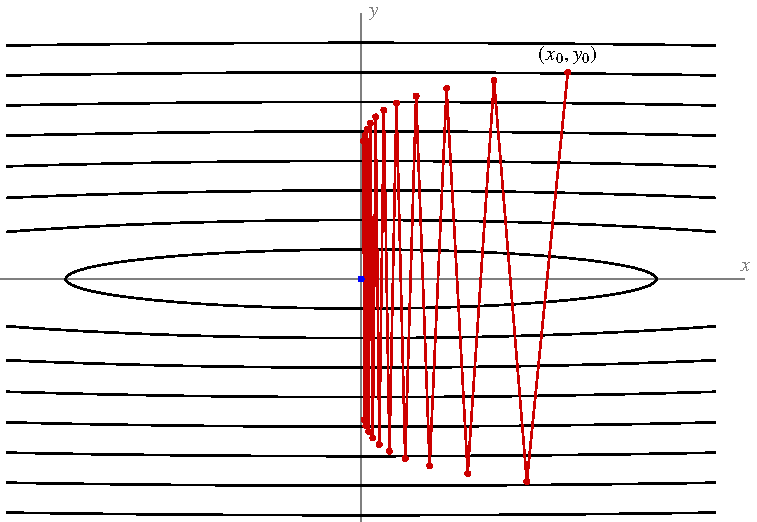
\includegraphics{chapters/070-direkt/images/abstieg.pdf{}
\caption{Gradientabstieg für die Funktion $f(x,y)=x^2+100y^2$.
\label{buch:direkt:gradient:fig:abstieg}}
\end{figure}

Zum Beispiel sind die Niveaulinien der Funktion
\(
f(x,y)
=
x^2+100 y^2
\)
sehr schmale Ellipsen, deren grosse Halbachse zehnmal grösser ist als
als die kleine Halbachse (Abbildung~\ref{buch:direkt:gradient:fig:abstieg}.
Der Gradient ist
\[
\operatorname{grad} f(x,y)
=
\begin{pmatrix}
2x\\
20y
\end{pmatrix},
\]
die zweite Komponenten des Gradienten ist also zehnmal grösser als
die erste, solange $x$ und $y$ von der gleichen Grössenordnung sind.
Der Gradientabstieg führt daher auch vor allem Schritte in $y$-Richtung
durch.
Die Grösse dieser Schritte entscheidet darüber, wie erfolgreich die
nachfolgenden Schritte sein werden.
Nur wenn die schmale Zone nahe der $x$-Achse getroffen wird, in der
die $y$-Koordinate etwa eine Grössenordnung kleiner ist als die
$x$-Koordinate, wird der nachfolgende Abstiegsschritt eine bedeutende
$x$-Komponente haben.
Nur wenn der erste Schritt genau die grosse Halbachse der Ellipse
trifft, wird der nächste Schritt auf der $x$-Achse bleiben.
Die Wahl der Schrittgrösse hat daher ganz entscheidenden Einfluss
auf die Konvergenzgeschwindigkeit.

Für quadratische Extremalprobleme ist es möglich, die Abstiegsschritte
optimal zu wählen, dies ist das gausssche Verfahren der konjugierten
Gradienten zur Lösung linearer Gleichungssysteme.
Für beliebige nichtlineare Problem steht dieses jedoch nicht zur
Verfügung.

Ein wichtiger Spezialfall ist die Lösung gewisser partieller
linearer Differentialgleichungen erster Ordnung, wie sie sich als
Euler-Ostrogradski-Differentialgleichungen ergeben.
Solche Differentialgleichungen können in der Form
$Du=f$ mit einem geeigneten Differentialoperator $D$
geschrieben werden.
Viele partiellen Differentialgleichungen der mathematischen
Physik und in Ingenieuranwendungen sind von dieser Art.
Statt wie im Verfahren von Ritz ein Minimum des Funktionals zu
suchen, versucht das Verfahren von Galerkin eine Ersatzgrösse
zu bestimmen, die Aufschluss darüber geben kann, in welche Richtung
die Lösung verbessert werden kann.

Dazu wird eine Menge von orthonormierten Funktionen $u_k$,
$k=1,\dots,n$ gewählt und es wird eine Lösung der Gleichung
\[
D\biggl(\sum_{k=1}^n c_i u_i\biggr) = f
\]
gesucht.
Die Differenz der beiden Seiten zeigt, wie ``falsch'' die bisher
gefundene Näherung der Lösung ist, sie zeigt aber nicht, wie gut
sich die Abweichung überhaupt korrigieren lässt.
Da man aber nur eine durch die Funktionen $u_k$ darstellbare
Lösung sucht, reicht es auch herauszufinden, wie gross die durch
$u_k$ darstellbare Komponente der Abweichung ist.
Dazu bestimmt man die sogenannten Residuen
\[
\biggl\langle
u_k,
D
\sum_{i=1}^n c_iu_i
-f
\biggr\rangle
\]
und versucht die Koeffizienten ${\color{darkred}c_i}$ so anzupassen,
dass der Fehler verschwindet.
Man löst also eigentlich das lineare Gleichungssystem
\[
\sum_{i=1}^n
\langle u_k,Du_i\rangle
c_i
=
\langle u_k,f\rangle
\]
mit Koeffizientenmatrix $A$ und rechter Seite $b$ mit Einträgen
\[
a_{ki}
=
\langle u_k,Du_i\rangle
\qquad\text{und}\qquad
b_k
=
\langle u_k,f\rangle
\]
für die Unbekannten ${\color{darkred}c_i}$.
Diese Vorgehensweise ist als das {\em Verfahren von Galerkin} bekannt.
\index{Galerkin-Verfahren}%
\index{Verfahren!von Galerkin}%
